\documentclass[a4paper,12pt, listof=totoc]{report}

\usepackage[T1]{fontenc}
\usepackage{arial}
\renewcommand{\familydefault}{\sfdefault}

\usepackage[spanish]{babel}

\usepackage[utf8]{inputenc}

\usepackage{setspace}

\usepackage{float}

\usepackage{graphicx}

\usepackage{geometry}
\newgeometry{ bottom=2.5cm, top=2.5cm, left=3cm, right=2.5cm}

\usepackage{pdfpages}

\usepackage{titlesec}
\newcommand{\sectionbreak}{\clearpage}
\usepackage{hyperref}


\pagestyle{plain}

\usepackage{etoolbox}

\doublespacing

\author{
  Fernando Garcia Corona\\
  \texttt{https://github.com/FerCorona/crown}
}

\begin{document}
	
	\pagenumbering{Roman}
	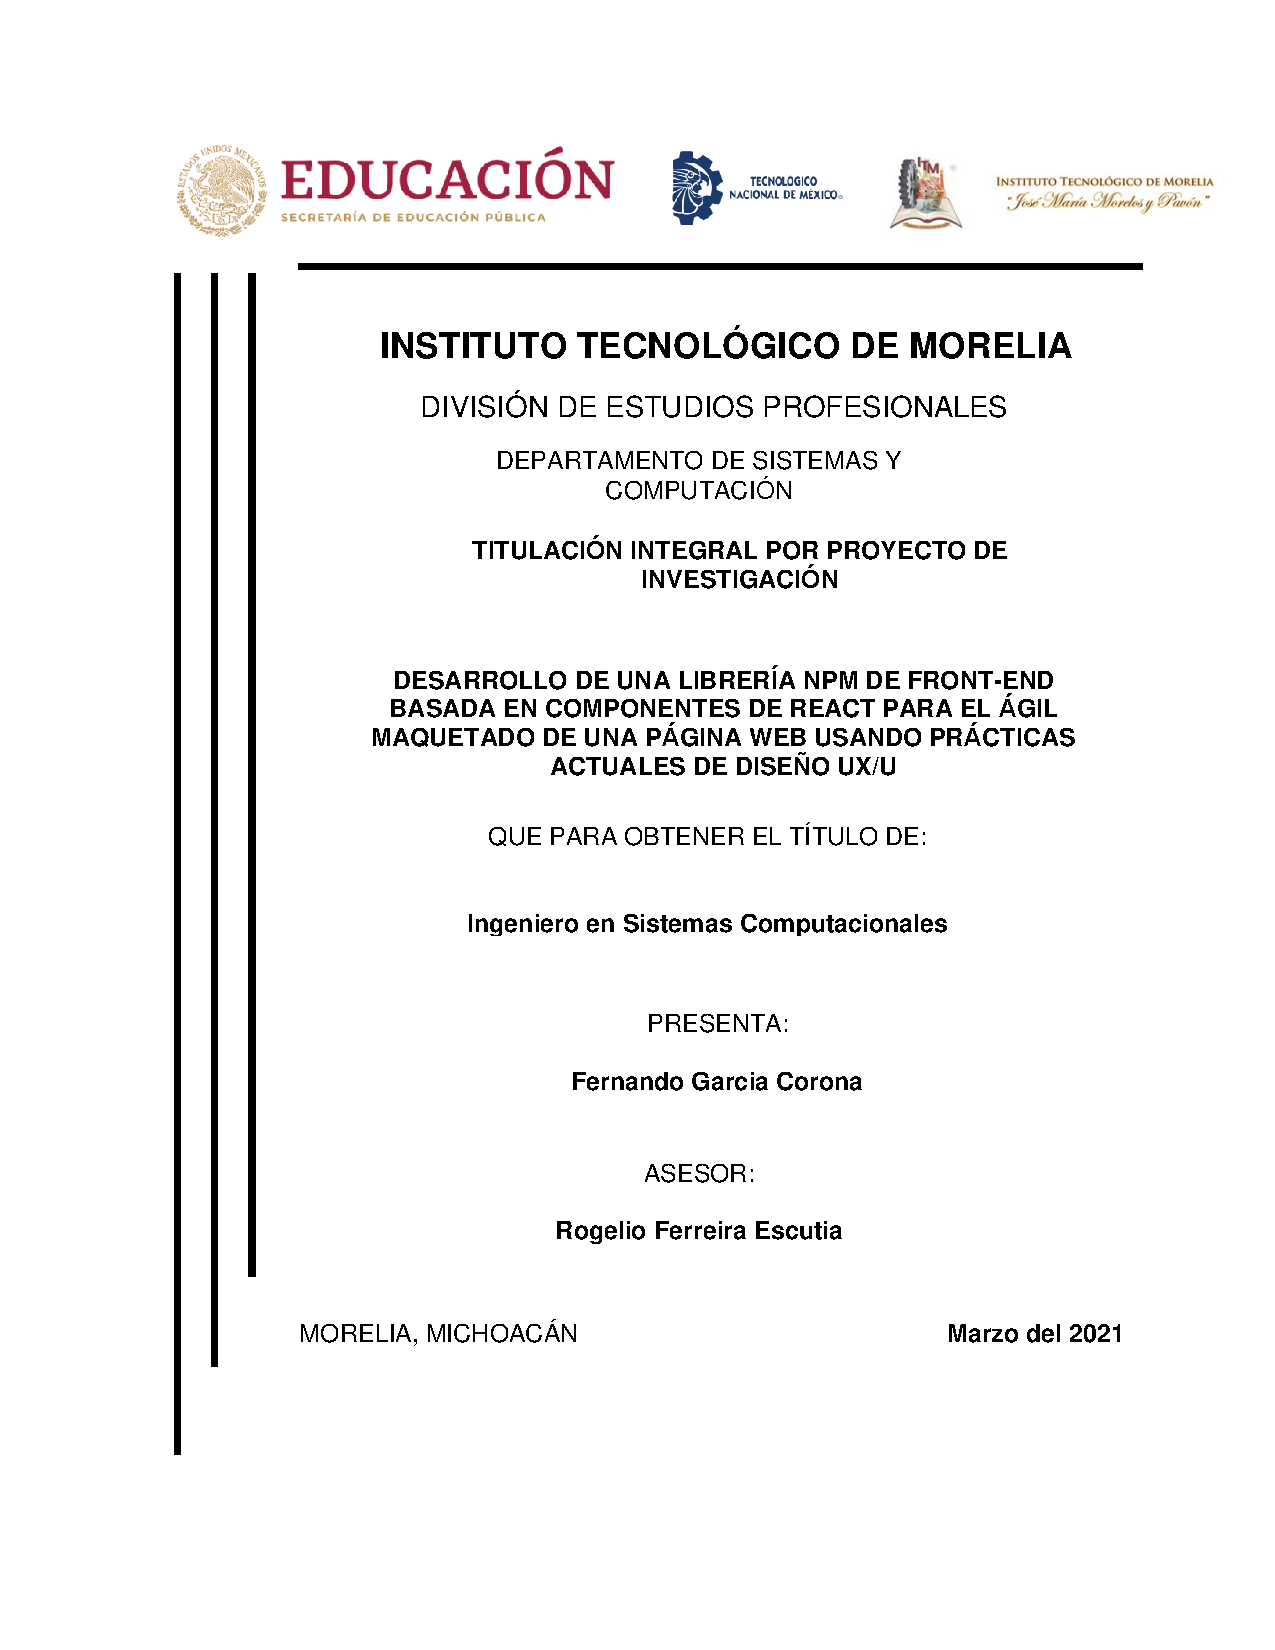
\includepdf[pages=-]{portada.pdf}
	
	\chapter* {Copia del Oficio de Impresión definitiva División de Estudios }
	
	\chapter* {Copia del Oficio de Impresión definitiva Sinodales}
	
	\chapter* {Agradecimientos }
	
	\tableofcontents
		
		\listoffigures
		
		\chapter {Introducción}
		\pagenumbering{arabic}
			JavaScript cuenta con un gestor de paquetes llamado NPM, este es encargado de gestionar el contenido, cada uno de los paquetes son  implementados en proyectos Web.
Actualmente no es común encontrar alguna página Web en el que el cien por ciento sea desarrollado por un solo equipo, ya que existen herramientas que son fáciles de agregar y no tienen costo alguno.
NPM es el conjunto de paquetes que los desarrolladores desean proveer a la sociedad para su libre uso.
Es por esta razón que durante el presente documento se desea desarrollar otra herramienta para que las personas, tengan otra alternativa fácil de usar y que puedan ser implementada en sus proyectos rápidamente.
Durante el presente documento se describe el proceso para desarrollar una librería. 
Se cubrirá la creación del ambiente requerido, instalación de paquetes, creación de ficheros y configuración de los mismos. 
También se describira el desarrollo de cada uno de los componentes que se planea tener, se mostrará parte del código fuente que hace que estos funcionen correctamente, y los requisitos necesarios para que trabajen de manera adecuada. 
Se dará una pequeña introducción al framework React, ya que la presente librería trabaja en conjunto con el.
En el desarrollo de la librería se implementara una guía de estilos de código para que el código sea un estándar, esto se logra usando la guía de estilos propuesta por Airbnb \cite{airbnb}que es una de las más usadas ya que actualmente obtendremos como resultado final un código fuente consistente en todo el desarrollo del proyecto, también nos ayuda a tener un código mucho más legible y en la medida de lo posible eficiente, aunque en algunos casos nos vemos restringidos al tener un estilo de programación que difiere , así cualquier persona interesada podrá colaborar para aumentar las funcionalidades una vez una primera versión aquí desarrollada esté lista.
Al terminar el desarrollo se tomará el tema de los test que trata de la manera en que se comprueba el correcto funcionamiento de lo aquí hecho.
Finalmente se muestra la manera de usar los componentes aquí desarrollados, la manera de instalar la librería y la correcta manera de implementarla.

Esta librería está creada con base en React, motivo por el cual se crean componentes como campos de texto, imágenes, tablas y varios más elementos que pueden ser implementados como cualquier componente de React. 

Los componentes que aquí se desarrollan están estilizados en base a gusto personal pero siguiendo prácticas de diseño de interfaces y experiencia de usuario, dando la posibilidad de que cuando se implemente algún elemento a este se le puedan dar parámetros básicos como podrían ser el color o el tamaño.

También cada uno de los componentes están conectados con el estado de React permitiendo un veloz desarrollo de la página Web que se desea hacer con esta librería, esto significa que al realizar el maquetado automáticamente ya se tendrá un control de los datos.

Al finalizar el desarrollo se tendrá una librería probada y publicada en el gestor de paquetes NPM, para que cualquier persona pueda acceder a esta.
			
		\chapter {Justificación }
			Actualmente, el desarrollo de páginas Web es una de las oportunidades de empleo con mayor demanda dentro del área de la informática, en los principales buscadores de empleo  \cite{work} se pueden encontrar una área de oportunidad para ejercer. El desarrollo Front-End, de páginas Web, es una de las subáreas más buscadas por las empresas que implementan servicios basados en Web, o que de alguna manera consumen algún producto. 
El famoso sitio Stackoverflow  \cite{stackOverflow}realiza una serie de estadísticas anuales en las cuales da a conocer los lenguajes de programación en los cuales ellos obtienen un mayor número de búsquedas y respuestas. Las estadísticas muestran que, durante el transcurso del año pasado (2020), el lenguaje más usado por la comunidad de desarrolladores profesionales es Javascript. 
Por otra parte, dentro esta serie de estadísticas se cuenta con un apartado para los marcos de trabajo, en el cual encontramos que en segundo puesto está React, solo por debajo de jQuery el cual puede ser empotrado dentro de React.  Finalmente se encontró que la biblioteca número uno es Node.js. 
El desarrollo Front-End  \cite{frontEnd}de páginas Web consiste en hacer la visualización que tenemos cuando ingresamos a algún sitio desde nuestro navegador, para esto es necesario que el programador que realiza la tarea tenga conocimientos básicos de HTML, CSS y JavaScript, para que sea posible construir una Web sencilla. Cabe destacar que un desarrollador Front-End no es el encargado de diseñar la experiencia de usuario ni tampoco el diseño de interfaz gráfica, ya que para esto existen otras disciplinas especializadas, pero en caso de tener conocimiento en el área puede agregar una herramienta que puede combinarse y agregar habilidades.
\newline
En la medida que una Web escala, esta tiende a aumentar su complejidad de desarrollo si no se comienzan a usar bibliotecas o marco de trabajos, que nos permiten a tener un trabajo más limpio, organizado, seguro y modulable. 
Como se mencionó anteriormente Javascript es usado tanto de manera profesional como con otros fines como los académicos, este lenguaje cuenta con un gestor de paquetes denominado NPM  \cite{npm},  que permite que se agreguen miles de funcionalidades extras a tu proyecto, NPM consiste en un cliente de líneas de comandos con el cual es posible agregar a nuestro proyecto paquetes, estos paquetes son de utilidad porque podemos reusar código que alguien más ya desarrollo, probó y decidió compartirlo, haciendo que el trabajo sea más ágil.  De igual manera nosotros podemos aportar publicando nuestra biblioteca. Dentro de NPM contamos con miles de bibliotecas de código abierto.  
Teniendo esto en cuenta, nos da la posibilidad de tener nuestra propia biblioteca y publicarla, para que personas a las cuales tienen alguna necesidad, pero no cuentan con el tiempo de ejecutarla puedan acceder a la nuestra, e incluso nosotros mismos usarlas en posteriores proyectos. 

El desarrollo de software de código abierto \cite{openSource} consiste en publicar algún tipo de herramienta propia, el cual será de licencia pública para que más personas puedan acceder al código fuente, si lo desean podrán usarlo o adecuarlo a sus necesidades. 
Anteriormente se mencionó un marco de trabajo de Front-End llamado React, este es mantenido por Facebook desde mayo del 2013 que fue su fecha de publicación, en la actualidad tiene más de mil contribuidores según lo indica el repositorio oficial. 
Algunas de las particularidades de React  \cite{reactOreilly}es que nos motiva a crear componentes que pueden ser utilizados más veces, y de esta manera tener una menor cantidad de código y más reutilizable. 
Nos deja crear una aplicación en una sola página que de ser de una manera tradicional y a gran escala se convertirían en una tarea imposible.
\newline
Por el uso desmedido de cada una de las tecnologías que se han mencionado nace la razón por la cual se desea desarrollar una biblioteca de NPM, la cual ayudará grandemente a la comunidad de desarrolladores de páginas Web y esto principalmente a las personas que cubren el rol de programadores Front-End. 
Esta biblioteca permitiría a los desarrolladores agilizar su carga de trabajo, poniendo a su alcance un conjunto de elementos usados en el desarrollo Front-End, alguno de ellos son botones, textos, etiquetas de texto, tablas, checkbox, radio botones, etc.  Los cuáles serán elementos definidos, que contarán con una definición de estilos \cite{scss} (CSS) establecidos, cada componente permitirá al desarrollador modificar parámetros básicos como el color, el texto y acción que va a realizar, esto con el fin de adaptarlo a las necesidades propias del proyecto en el que se va a hacer la implementación de la biblioteca.  
Otra ventaja por parte de la biblioteca es que esta estará basada en prácticas modernas del diseño UI/UX, como lo es Mobile First \cite{mobileFirst} Indexing (ideología de Google), que nos pide enfocar el diseño de cualquier Web primero para dispositivos móviles, ya que afirman que es en el mercado el cual consume más contenido Web, ayudándonos a no requerir un conocimiento avanzado sobre el diseño de interfaces gráficas. 
Esto nos dará la garantía de la experiencia del usuario, lo que significa que el usuario sabrá que está haciendo en todo momento, y también estaremos otorgando un diseño de interfaz moderno.
Ya que el diseño de cada elemento de la biblioteca estará diseñado para ser fácil de usar para el desarrollador y usuario final y garantizar que el resultado del desarrollador sea el mejor para el usuario final.
Finalmente, además de los elementos básicos que incluirá la biblioteca, tendrá más elementos que permitirán aún más la eficiencia, contendrá otros elementos compuestos como formularios, tarjetas, alertas, pies de página, menús de navegación, elementos deslizables. 

La última parte de la biblioteca consistirá en elementos aún más compuestos, denominados plantillas que consiste en pantallas de login, registro, página de inicio entre otras. Abriendo la posibilidad que más personas puedan aportar creando sus propias plantillas, y crear una comunidad de desarrollo.  
Debemos tomar en cuenta que este proyecto no se puede clasificar dentro del área de los marco de trabajos ya que para ser parte de, es necesario contemplar toda la estructura necesaria dentro de una página Web, modelos, vistas y controladores (MVC). Nuestro proyecto está focalizado en las vistas, por lo cual puede clasificarse como biblioteca.  
  
Con el uso de esta biblioteca reduciremos el tiempo de desarrollo, ya que no comenzaremos a escribir HTML y  CSS desde cero, tendremos una base común sobre la cual podemos seguir. Todo el equipo tendrá los mismos estilos y evitaremos que nuestra Web tenga discrepancias dentro de los diferentes módulos o vistas que tiene nuestra Web. 
Al usar esta biblioteca nos aseguraremos de que las vistas de nuestra aplicación Web puedan mirarse estéticamente iguales y tendemos la seguridad de que luzca de la misma forma en Chrome, Safari Firefox o un mayor número de navegadores, no importa si es una versión actual o una más antigua. 
Con esta biblioteca evitamos el tiempo de aprender un nuevo marco de trabajo, ya que funciona sobre React y los conocimientos necesarios son saber React. 
Tendríamos una organización predeterminada para todo el proyecto en el que se implementa, teniendo uniformidad en el desarrollo y en la interfaz gráfica, aumentando la agilidad en el trabajo y de manera proporcional reduciendo el tiempo y primordialmente el costo que implica, también reducirá el mantenimiento, así como los posibles errores. 
Debemos tomar en cuenta que el número de personas que participan en el desarrollo de un software es variado, pero regularmente este es mayor a uno, por lo que es conveniente que el código sea claro, legible y reutilizable para que el mayor número de personas que están involucradas, para que puedan trabajar en la mayor parte del proyecto sin problemas en caso de que exista un cambio de roles, es por lo que usar una biblioteca estandariza el trabajo. 
Las bibliotecas cumplen con gran cantidad de pruebas, para que no surjan problemas y sean impedimento al implementarlas, esta no será la excepción al incluir pruebas de validación, así también se eliminan errores en el proyecto donde se implementan. 
  
Lamentablemente como en todo marco de trabajo y biblioteca existe la desventaja a que al implementarlo este te fuerza a verte limitado con respecto a la cantidad de configuración y personalización que podemos editar \cite{newTech}. Otra cosa por tomar en cuenta es que no se necesita aprender una sintaxis específica para usar esta biblioteca, pero es necesario conocer la sintaxis que se usa con React, ya que esta biblioteca es basada en React, y es necesario conocer los conceptos básicos como el uso de componentes y el paso de elemento. Al usar una nueva biblioteca es posible que sientas que estás perdiendo el tiempo al incorporarlo en proyectos, debido al tiempo de aprendizaje. También no se encuentra recomendable agregar la biblioteca en un proyecto que ya está avanzado, y no lo es por el funcionamiento o incompatibilidad de bibliotecas, esto es más bien, porque no es viable visualmente ya que se encontrara elementos y vistas distintas unas entre otras, esto, si no se decide actualizar los elementos existentes lo cual aumenta el tiempo de desarrollo.


Debemos considerar que al agregar una capa software extra a nuestro Proyecto aumenta en tamaño, ya que además del peso de React que es necesaria para usar esta biblioteca debemos contar el peso de nuestra biblioteca en sí, aunque no todas  las tecnologías  mencionadas son agregadas en la versión que estará alojado en el proyecto, ya que por ejemplo Webpack \cite{webPack}, solo es usado durante el desarrollo.

Al usar la presente biblioteca se acorta el trabajo necesario, que es requerido después de que el maquetado de nuestra página Web está listo, ya que a diferencia de otras bibliotecas  como Material Design solo se enfocan el maquetado pero esta biblioteca se involucra en la funcionalidad de los componentes.

Una vez un componente de esta biblioteca, se implemente,  este no necesitará trabajo extra, el componente estará listo para ser utilizado, por ejemplo para el componente de entrada de texto estará directamente conectado con el estado de React, eso significa que cuando necesitemos el dato introducido ya lo tendremos listo, y no como en React simple que debemos procesar el input para poder obtener el dato.

Esto deja la biblioteca como una opción híbrida entre el maquetado simple conformado por HTML, CSS etc. y el procesamiento de los datos con JavaScript y PHP.

\newpage
		
		\chapter {Objetivos }
			\section {Objetivos Generales}
				Desarrollar una librería para el desarrollo de páginas Web, especialmente para el área de front-end, publicada en el gestor de paquetes de JavaScript “NPM”, usando el framework React, permitiéndonos la utilización de componentes para facilitar, agilizar y mejorar el maquetado de una página Web, incluyendo prácticas de diseño UI/UX que permiten que el usuario llegue a entender el funcionamiento de la aplicación sin que se requiera un entrenamiento de la misma, haciendo el sito que implemente la librería fácil de usar y atractiva visualmente. 

			
			\section {Objetivos Específicos} 
				  \begin{itemize}
 \item Desarrollar una librería para el desarrollo Front-End de páginas Web.
 \item Publicar la biblioteca para su uso con el gestor de paquetes de JavaScript \cite{javascript} llamado NPM.
 \item Usar el marco de referencia React que nos permite la creación de componentes reutilizables.
 \item Implementar Web-pack para garantizar el funcionamiento de la biblioteca ya que nos permite empaquetar y exportar todos los módulos y dependencias que incluye nuestra librería en un solo archivo para la correcta y ágil implementación. 
 \item Aunado a esto se utilizará Babel \cite{babel} que es un convertidor de código JavaScript a versiones anteriores, lo que nos permitirá una gran cantidad de compatibilidad con navegadores antiguos. 
 \item Para unificar nuestra sintaxis se usará ESLint el cual nos permite definir una guía de estilos para la librería, sobre esto se usará una guía de estilos ya definida y probada, la de Airbnb. 
   \end{itemize}
\newpage

		
		\chapter {Caracterización Del Área En La Que Se Participó  }
			El presente trabajo fue desarrollado para el uso libre y futura implementación en proyectos de software. Específicamente en el ambiente de la programación web, para su utilización en áreas en las cuales se usa como base la librería React, ya que nuestro trabajo funciona sobre React.
 \newline
  \newline
Esta librería se encuentra publicada en el gestor de paquetes de JAVASCRIPT llamado NPM. 
 \newline
  \newline
El rol que toma más partido en el uso de nuestra librería es el Front-end, ya que es el área que desarrolla la parte visual para el software. La librería brinda la facilidad de implementar elementos como botones, imágenes, campos de texto, etiquetas de texto, etc. de una manera simple y sin necesidad de darle un diseño a cada elemento al dar parámetros simples como el como pueden ser color y tamaño.

		
		\chapter {Problemas A Resolver Con Su Respectiva Priorización }
			La inspiración del presente proyecto yace como la solución al conjunto de problemas que se encontraron al estar desarrollando una página web.

\begin{itemize}

   \item \textbf{Personal} \newline Al estar desarrollando una página web es posible pertenecer a un equipo en el cual no te tiene un integrante del área de diseño encargado del diseño de interfaz y diseño de experiencia de usuario, el cual brinda el punto de partida para las personas que se encargan de la maquetación de una web, esto puede ser por que no se cuenta con los recursos monetarios para contratar a una persona o por inasistencia.  
   \item \textbf{Tiempo}\newline  Existen ocasiones en los desarrollos de software, en los que el tiempo previsto fue afectado al resolver otros problemas existentes. En esos casos el tiempo para tener una nueva funcionalidad se reduce o simplemente el tiempo estimado para terminar el trabajo fue erróneo. Al tener una librería ganas el tiempo que puedes perder si inicias desde cero. Otras veces se le da más peso a la funcionalidad y se considera un buen diseño y no quieres perder calidad.
   \item \textbf{Estandarización} \newline Cuando desarrollas una pieza de software, esta cuenta con múltiples colaboradores cada uno con distintas maneras de pensar y por consiguiente tu código tiene múltiples estilos de código.   Al usar esta librería se está estandarizando tu trabajo, y cualquier nuevo integrante o cualquier cambio en los roles del equipo puede adaptarse fácilmente.
   \item \textbf{Soporte}\newline  Al consumir los recursos de alguien más, estás garantizando que cualquier error que esto genere no serás el responsable de resolverlo.
   \item \textbf{Reinvención}\newline  Cuando ya existe alguna funcionalidad trabajando correctamente no es necesario desgastarse en volver a generar el trabajo.
\end{itemize}
			
		\chapter {Alcances Y Limitaciones }
				\section{Alcances}

Para el desarrollo del presente proyecto se contempla la implementación de un conjunto de elementos, que podrán ser integrados en cualquier proyecto en el que se use JavaScript y el gestor de paquetes NPM. Debe considerarse que al momento de instalar la presente biblioteca instalará forzosamente React.
 \newline
Se enlistan los primeros elementos que son considerados en el desarrollo. Los cuales son los elementos básicos y que al combinarlos es posible generar interacciones mayores.
 \newline
\begin{itemize}
\item Botón 
\item Campo de texto
\item Tabla
\item Etiqueta de texto
\item Radio botón
\item Switch
\item Imagen
\item Cuadro de selección
\item Radio botón 
\end{itemize}
 \newline
También se incluyen otros elementos que no son considerados como básicos pero son  igualmente utilizados, entre ellos se tienen los siguientes:
 \newline
 \begin{itemize}
\item  Alertas
\item Tarjetas de contenido
\item Formulario
\item Barra de navegación
\item Ventanas modales
\end{itemize}
\newline
 Finalmente con una complejidad mayor se tendrán vistas completas que pueden ser usados, estos son:
  \newline
 \begin{itemize}
\item  Formulario
\item Inicio de sesión
\item Registro de datos
\end{itemize}
\newline
El conjunto de elementos a desarrollar se tendrán debidamente funcionales y supervisados bajo un marco de pruebas de JavaScript, para esto se estará usando el marco de trabajo Jest así garantizando la funcionalidad esperada para los usuarios que desean usar la biblioteca, evitando los problemas que pudieran encontrar en los proyectos que lo implementaran. 
Cada elemento estará debidamente estilizado bajo consideración propia y los conocimientos adquiridos sobre la presente acerca de la experiencia de usuario y el diseño de interfaces.

\section{Limitaciones}
Actualmente se considera que gran parte de la planeación inicial pueda ser llevada al ambiente de producción, aunque actualmente ya se encontraron algunas limitaciones derivado al alto tiempo que se tomará durante el desarrollo y la documentación necesaria para los usuarios.
Esta limitación no afecta gravemente al desarrollo planeado inicialmente, ya que los elementos básicos se lograran tener listos al final del proyecto y se les asignará una mayor prioridad.
Los elementos que se planea terminaran afectados son los siguientes. 
\newline
\begin{itemize}
\item  Formulario
\item Inicio de sesión
\item Registro de datos
\end{itemize}
\newline
Anteriormente se planeaba tener una mayor cantidad de parámetros personalizables a los iniciales, pero esto toma gran cantidad de tiempo.
Ahora se considerarán sólo parámetros básicos necesarios para el correcto funcionamiento como el color y los datos a solicitar para el caso de la vista de registro.

  
		
		\chapter {Marco Teórico  }
			    \begin{itemize}
    
    	\item \textbf{Librería Front-end:} Una librería Front-end \cite{frontEnd2}es una herramienta que es agregada a nuestros proyectos, en este caso web, el cual incorpora elementos que otras personas o equipos ya desarrollaron, sumando funcionalidad a nuestra web, reduce el mantenimiento y el tiempo de desarrollo, algunas características que existen actualmente y pueden agregarse van desde gráficas, animaciones, mapas etc. 
      
       \item \textbf{NPM :} NPM \cite{npm} es un gestor de paquetes que nos permite agregar dependencias a cualquier proyecto basado en Javascript, esto es posible con un cliente de líneas de comandos que es útil para poner o quitar los paquetes que deseamos. La configuración consta de un archivo en el cual contiene una lista de las dependencias que se quieren instalar en nuestro proyecto. Actualmente existen miles de paquetes que pueden ser descargados de manera gratuita y de igual manera permite colaborar. 
       
       \item \textbf{ React :} React \cite{react} es una librería de Javascript para el desarrollo de interfaces de usuario (Front-end), famosa por la posibilidad de hacer fácilmente webs de usa sola página. React fue desarrollada por Facebook y con el paso del tiempo, conocidas empresas han empezado a implementarlo en sus proyectos. 
    React nos permite desarrollar de una forma más ordenada y con el menos código necesario. 
    Se considera que React no es un Framework en comparación con ANGULAR o EMBER porque no tiene cada una de las áreas que propone el modelo vista controlador, este solo se encarga de las vistas. 
    Uno de los puntos fuertes de React es que cuenta con un DOM virtual el cual es almacenado en memoria, esto provoca que cuando algo cambie este se va reflejado en memoria de una forma más rápida, después el DOM virtual será comparado con el DOM del navegador y solo actualizara lo que encuentre diferente. 
    React funciona en base a componentes que pueden ser reusados cuantas veces sea necesario, una forma fácil de entenderlo puede ser como la programación orientada a objetos al hacer una instancia de una clase, estos componentes pueden tener un estado, que es encapsulado por sí solo, de manera local por cada uno y puede ser actualizado.  
    
       \item \textbf{HTML  :}   HTML \cite{html} es un lenguaje con un conjunto de etiquetas que permite definir el contenido con el que podemos interactuar dentro de una página web. 
       
       \item \textbf{ SASS :} SASS \cite{scss} es un preprocesador de CSS, el cual nos ayuda a agregar características que no tiene CSS puro y que son propias de los lenguajes de programación como variables, funciones, herencia entre otros. Nos permite dedicar menos tiempo para mantener y crear el CSS y agrega la posibilidad de tener una organización modular. 
       
       \item \textbf{ Webpack :} Hace algunos años Javascript iniciaba como un lenguaje que nos permitía agregar interacción a nuestras páginas web, que anteriormente eran simplemente contenido estático.  Javascript nos permitía recuperar los datos que eran introducidos en formularios, podíamos mostrar ventanas emergentes o incluso agregar animaciones. Para agregar Javascript en nuestros archivos de HTML, se debía agregar la etiqueta <script>, donde se indicaba la ruta donde estaba almacenado nuestro archivo .js de Javascript.  
    Años más tarde se agregó soporte al lenguaje Javascript, para permitir hacer peticiones asíncronas a nuestros servidores, esto hizo que las empresas empezaran a ver como viable el desarrollo web, que previamente estaba enfocado en el desarrollo de escritorio, también hizo que los archivos .js empezaran a crecer en cantidad de líneas en nuestros proyectos, y se miraba reflejado en nuestros archivos .html los cuales empezaron a tener múltiples etiquetas <script>. Lo que significaba múltiples peticiones para obtener los archivos del servidor, esto agregaba una capa de complejidad, debido a la inclusión de múltiples archivos .js embebidos en un .html y al agregarlos se debe tener en cuenta el orden en que se listan, porque es posible que tengan dependencias entre ellos. Actualmente es posible comprimir los múltiples archivos .js para que sean menos peticiones al servidor (CDN).  Cuando un proyecto con Javascript crecía aumentaba el número de módulos que se agregan, pero no existía la forma de gestionarlos. Un problema que tenía Javascript es que los navegadores no soportan un sistema nativo de módulos por eso se agregaron Require.js y Common JS. 
    En base a esto nació Webpack \cite{webPack} que permite usar NPM como gestor de dependencias y soporta el sistema de módulos Common JS.
    Webpack permite modular nuestro código, para esto genera un grafo dado un punto de entrada, el punto de entrada es el nodo inicial de nuestro grafo, el grafo es generado con las inclusiones de elementos encontrados en los archivos, como son imágenes, archivos de CSS etc. Esto genera un archivo final en el que estará el empaquetado de nuestros archivos. 
    Webpack nos permite especificar cargadores para distintos tipos de archivos como imágenes, SCSS, CSS, HTML. JSX, etc. ya que nativamente solo admite archivos Javascript. 
    La configuración es dada por un archivo que se coloca en la raíz del proyecto.
    
       \item \textbf{Babel  :}   Babel \cite{babel} es un traductor de código Javascript, que permite convertir el código Javascript más moderno en alguna versión más vieja, esto nos proporcionó la capacidad de que nuestro código pueda ser ejecutado por más cantidad de navegadores, los cuales solo pueden interpretar versiones anteriores de Javascript. Por ejemplo, el siguiente código es usado en React para mostrar un texto. 
    \begin{figure}[H]
    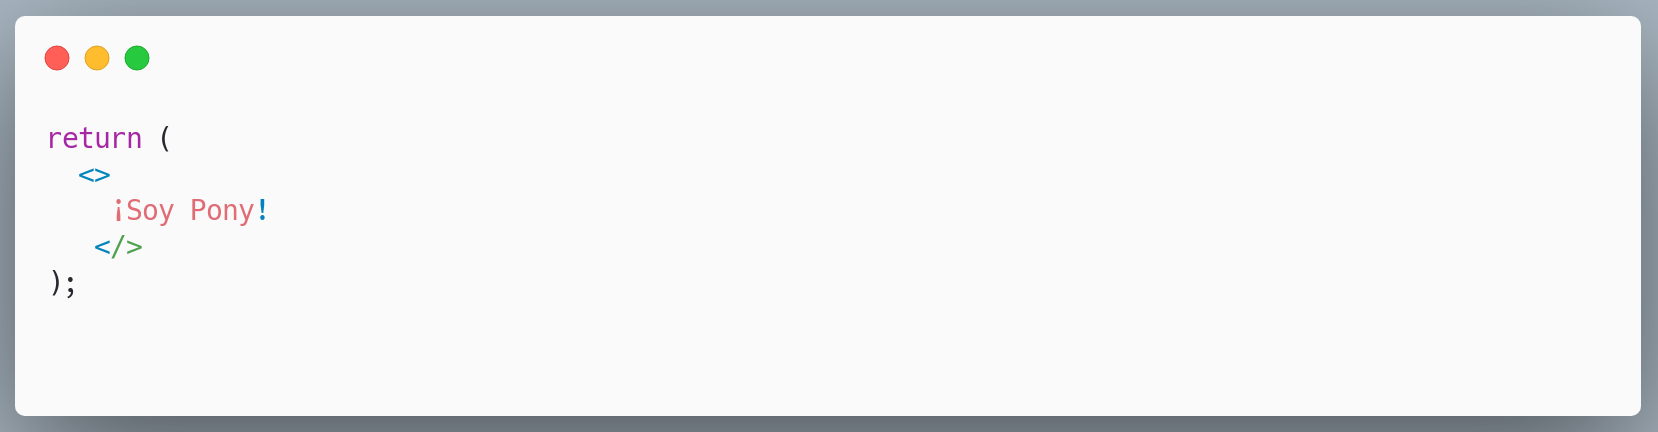
\includegraphics[width=1\textwidth]{./Imagenes/image16.png}
    \caption[Impresión de texto con React]{Impresión de texto con React}
    \end{figure}
       El código será convertido en el que se muestra En la figura 7.2, el cual es interpretada por un mayor número de navegadores. 
       \newline
       \newline
       \begin{figure}[H]
       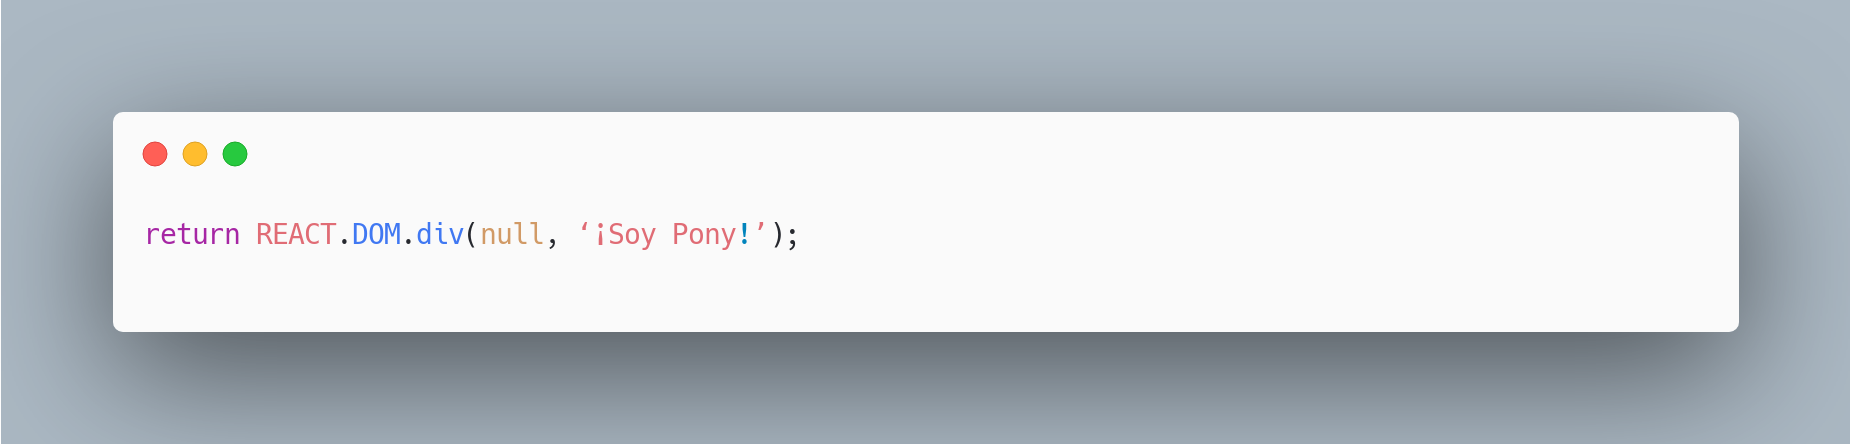
\includegraphics[width=1\textwidth]{./Imagenes/image5.png}
        \caption[Impresión de texto una vez el código es convertido]{Impresión de texto una vez el código es convertido}
       \end{figure}
       \newline
       \newline
       \item \textbf{ESLint :}ESLint nos permite definir una guía de estilos en nuestro código, lo que nos ayudará a tener un código limpio y claro para que sea fácil de editar y mantener, podemos agregar guías de estilos una de ellas es la de Airbnb, que es una de las más usadas. 
       
    \end{itemize}
		
		\chapter {Procedimiento Y Descripción De Las Actividades Realizadas}
			        El objetivo de desarrollo de la presente librería se basa en el siguiente principio, “ cuando un elemento sea actualizado, sea un botón, cuadro de estado, entrada de texto, etc. el componente regresará un objeto el cual tendrá el nombre del elemento y el nuevo valor para que este sea actualizado en el state de React ”.  Con esto deseamos generar el  flujo de la Figura 8.1.
        
               \begin{figure}[H]
           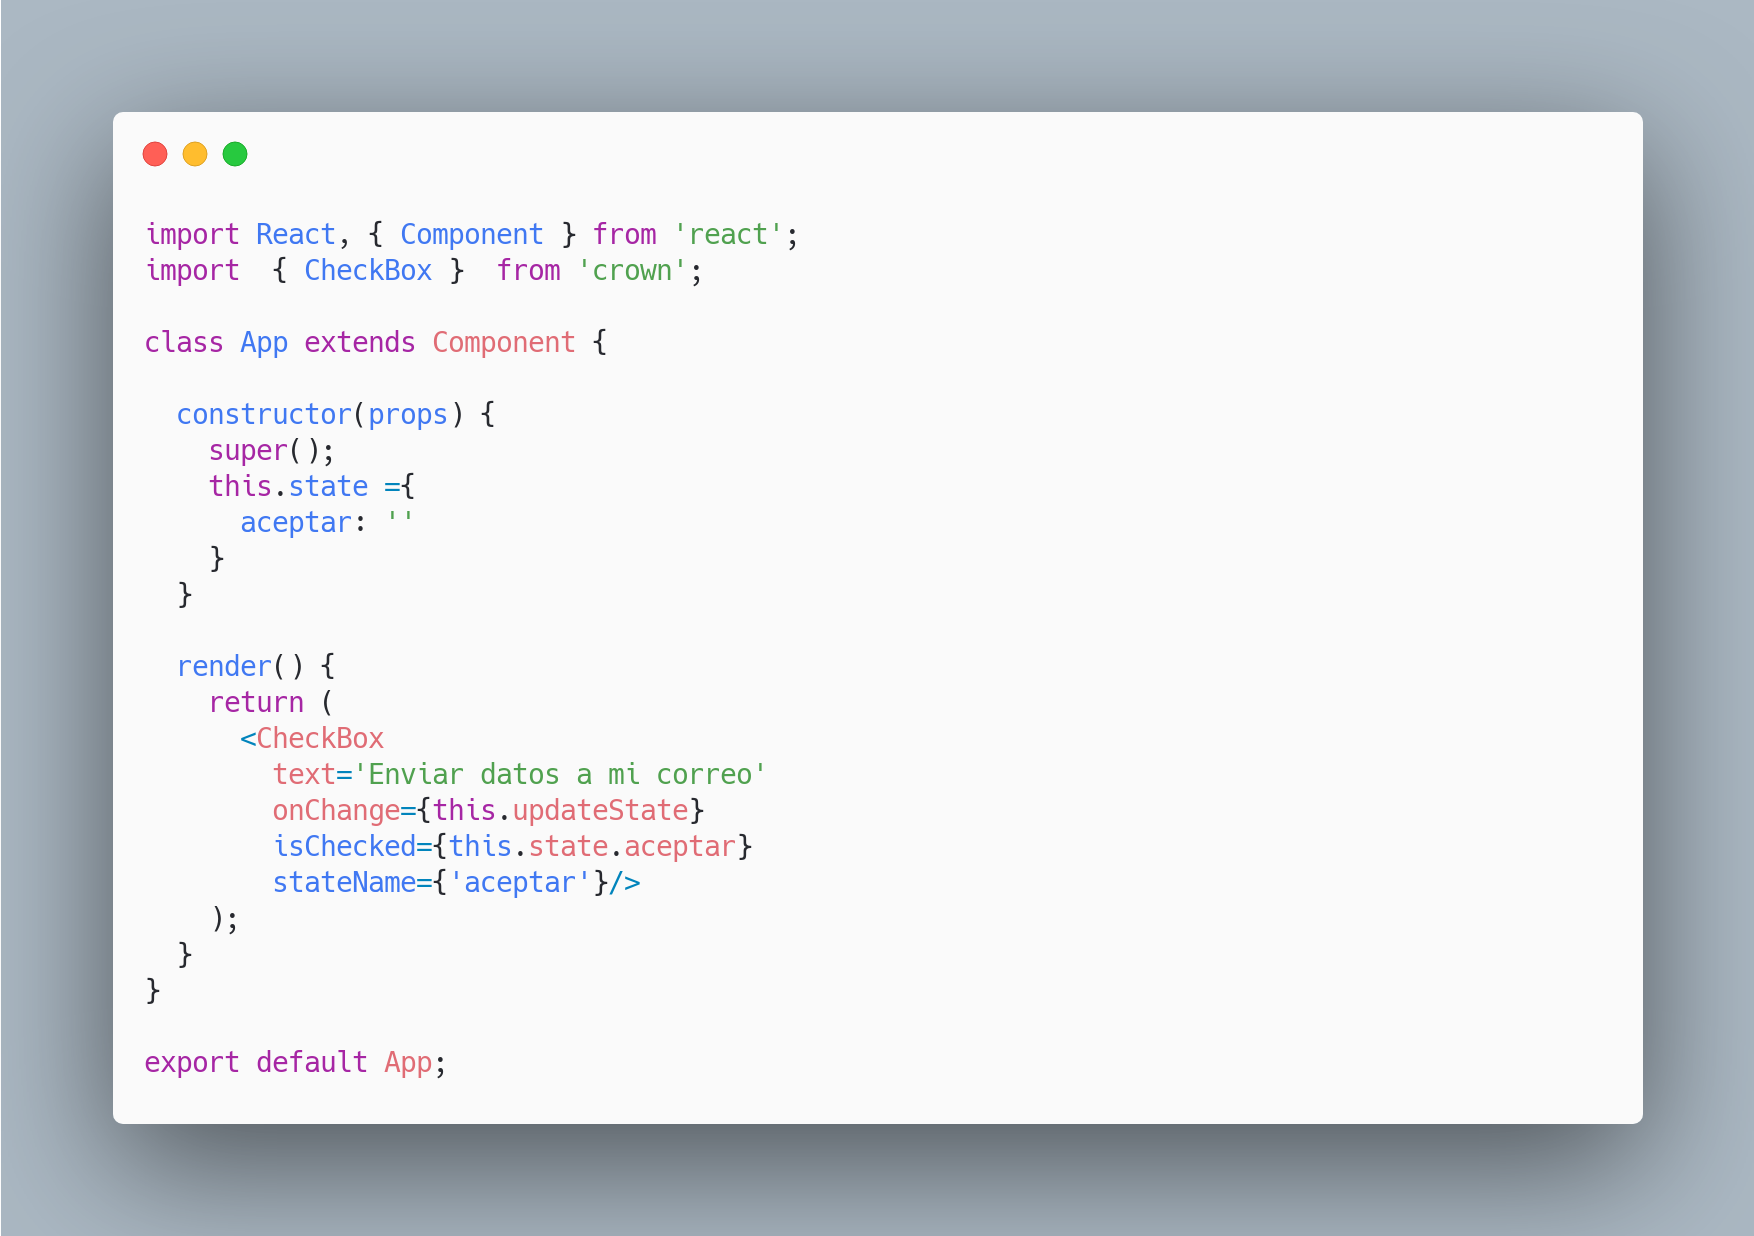
\includegraphics[width=1\textwidth]{./Imagenes/carbon-8.png}
           \caption[Resultado esperado de la librería]{Resultado esperado de la librería}
             \end{figure}
        
        Importamos el elemento CheckBox desde “crown” dentro de el método render en return  ponemos el componente CheckBox y le damos los  siguientes  props.
        
        \begin{itemize}
        	\item \textbf{onChange:} Función que actualiza el estado, que definiremos adelante.
        	\item \textbf{isChecked::} Ponemos el valor de “aceptar” que está en el estado.
        	\item \textbf{stateName:}  Es el nombre ( y no el valor como en isChecked ) con el que identificamos el elemento en el estado. 
        \end{itemize}
        
        \newline
        Dentro del componente CheckBox se devuelve un objeto como el que se muestra en seguida.
        \begin{figure}[H]
         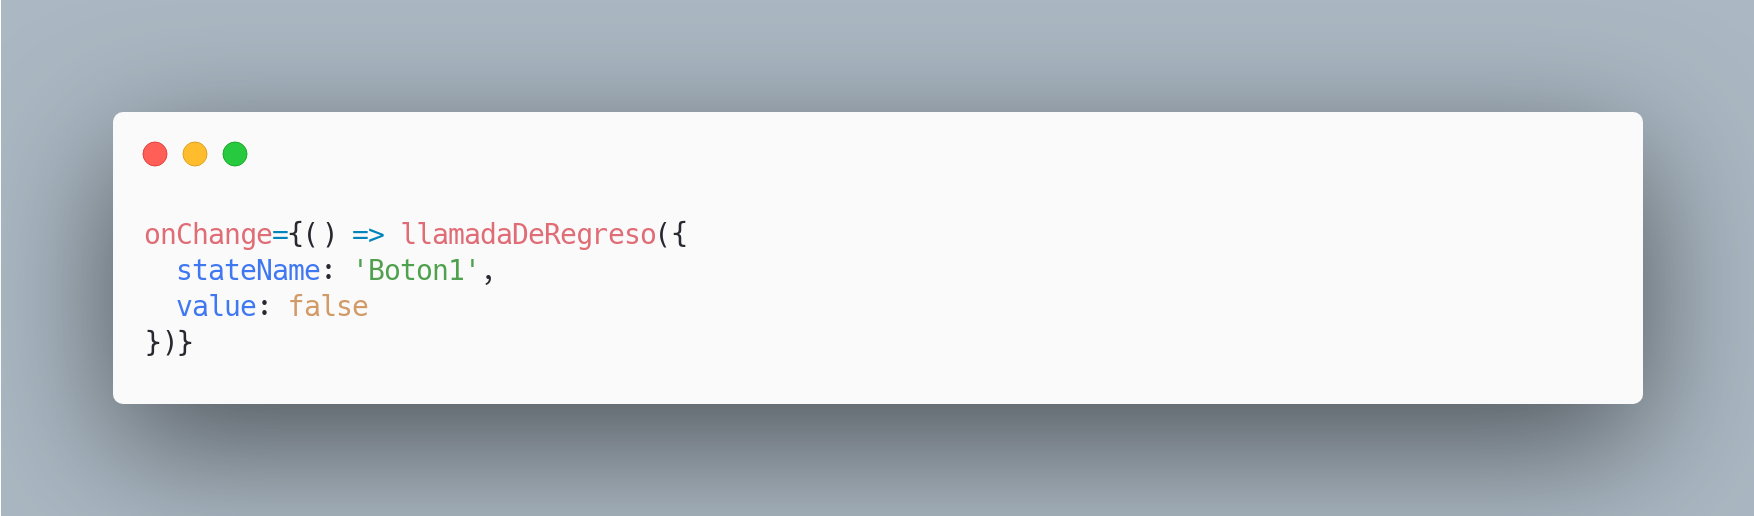
\includegraphics[width=1\textwidth]{./Imagenes/carbon-6.png}
         \caption[Resultado de la llamada]{Resultado de la llamada}
             \end{figure}
        \begin{itemize}
        	\item \textbf{onChange:}  Este es el evento que se ejecuta cuando una acción es disparada, por ejemplo cuando haces click en un CheckBox.
        	\item \textbf{llamadaDeRegreso:} Es la función que recibe el componente, y cuando se hace click en un CheckBox este, por defecto llama la acción que está dentro del evento onChange. En este caso llama a llamadaDeRegreso.
        	\item \textbf{stateName:}  Es el nombre ( y no el valor como en isChecked ) con el que identificamos el elemento en el estado. 
        	\item \textbf{value:}  Este dato almacena el valor actualizado del elemento, esto define si el CheckBox está seleccionado o no.
        \end{itemize}
        \newline
        Esto facilitará a tener una única función ( Figura 8.3 ) capaz de actualizar todos los elemento que agregamos ya que contamos con el nombre,  que es con el que se identifica en el estado y también el nuevo valor.
        \begin{figure}[H]
         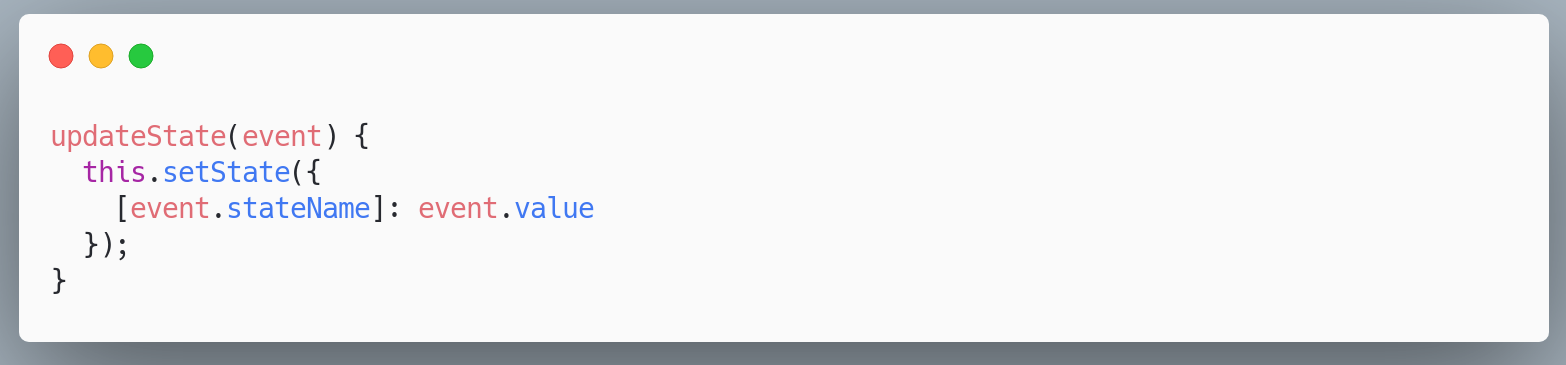
\includegraphics[width=1\textwidth]{./Imagenes/carbon-7.png}
         \caption[Actualización del estado]{Actualización del estado}
             \end{figure}
        \newline
        
        \end{enumerate}
			
			\section {Creación Del Ambiente De Desarrolo}
				    \subsection{Ambiente De Desarrollo}
    Durante el desarrollo de la presente librería se usó el sistema operativo MacOS, con la terminal que se incorpora por defecto en el mismo.
    El primer paso que se debe realizarse es colocarse en el directorio en el que se desea trabajar, esta librería se sitúa en la carpeta Documentos durante el desarrollo, usando el comando de la Figura 8.4 es posible cambiar de directorio, ejecutandolo en la terminal.
    
    \newline
     \begin{figure}[H]
     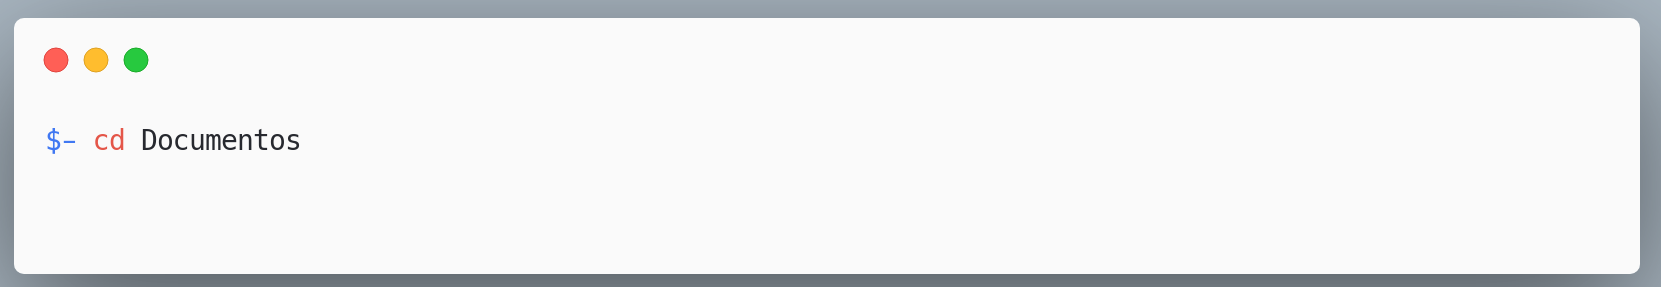
\includegraphics[width=1\textwidth]{./Imagenes/image15.png}
     \caption[Moverse entre directorios]{Moverse entre directorios}
         \end{figure}
Después se creó la carpeta de desarrollo son el siguente comando. Se llamó de manera simbólica como “crown”, que significa en español “corona”.
     \begin{figure}[H]
    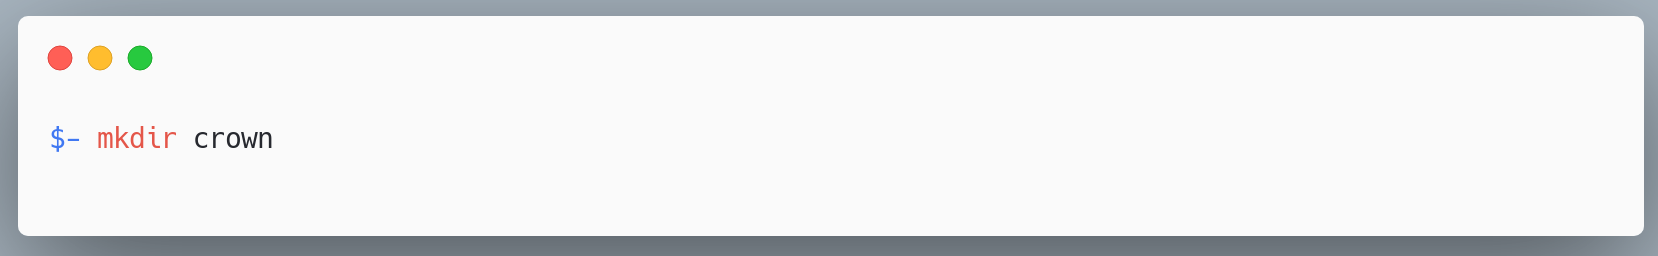
\includegraphics[width=1\textwidth]{./Imagenes/image7.png}
     \caption[Crear nuevo directorio]{Crear nuevo directorio}
         \end{figure}
    
    Dentro de esta carpeta debemos crear dos carpetas, una tendrá el código fuente, y la otra tendrá el resultado del código procesado que se importará por otros proyectos, con la ayuda del siguiente comando.
    \newline
     \begin{figure}[hbt!]
    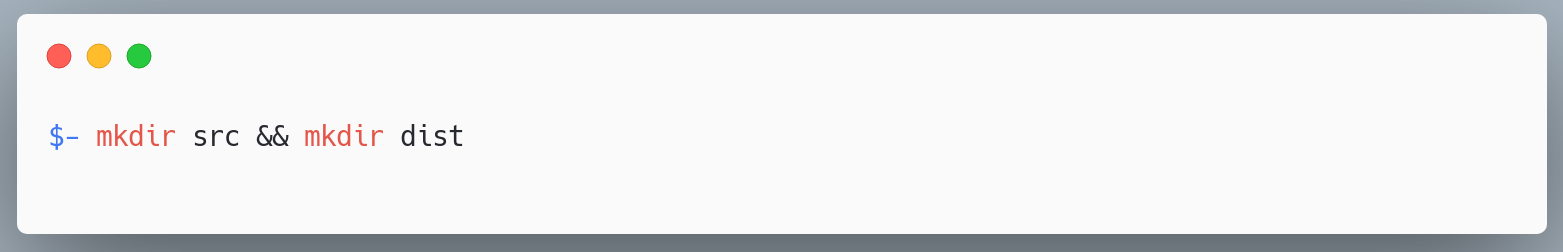
\includegraphics[width=1\textwidth]{./Imagenes/image37.png}
     \caption[Crear nuevos directorios]{Crear nuevos directorios}
         \end{figure}
    \newline
    \newline
    
    \subsection{Inicialización Del Archivo NPM}
    Se continúo inicializando el archivo de NPM, el cual nos sirve para llevar el control de las dependencias de JavaScript que se vayan agregando, esto ejecutando el siguiente comando.
    \newline
    \newline
     \begin{figure}[H]
    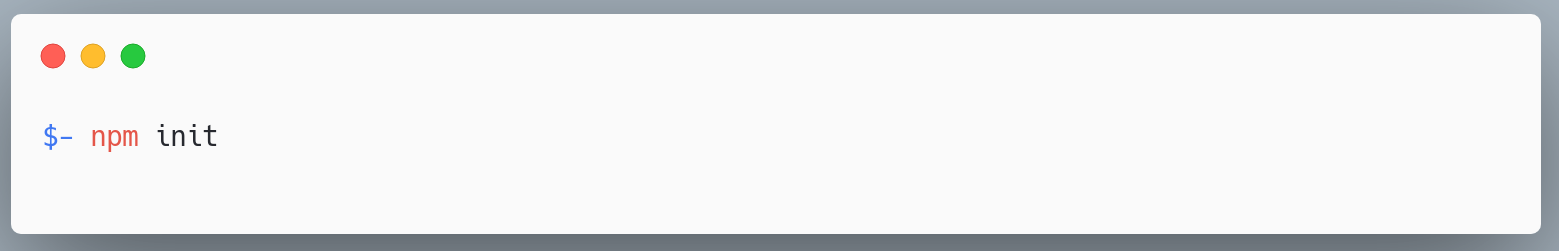
\includegraphics[width=1\textwidth]{./Imagenes/image11.png}
     \caption[Inicializar NPM]{Inicializar NPM}
         \end{figure}
    
    \newline
    \newline
    Al introducir el comando anterior este preguntara por una lista de datos necesarios, para tener el control de los paquetes, estos son los siguientes datos que se deben proporcionar:
    \begin{itemize}
    \item \textbf{Nombre del paquete:} Este es el nombre simbólico con el cual se puede identificar el paquete dentro del buscador de NPM, por lo tanto, es el nombre con el que nuestro paquete será encontrado.
    \item \textbf{Versión del paquete:}Con esta opción controlaremos la versión, y en caso de que se agreguen funcionalidades o se resuelva algún error, tendremos una manera de actualizar en los proyectos que incorporen esta librería.
    \item \textbf{Descripción del paquete: }Daremos a las personas una muy breve explicación acerca del uso que puedes obtener con nuestra librería.
    \item \textbf{Punto de entrada del paquete:} Es el directorio el cual será importado cuando agreguemos nuestra librería a otros proyectos, este podrá incluir la lógica o que solamente sea el nodo inicial de todo nuestro código.
    \item \textbf{Comando de prueba:} Dentro de este archivo nos permite incluir comandos que afectan a nuestra librería, en este caso, este comando nos sirve para ejecutar una serie de pruebas, para usar antes de publicar una nueva versión.
    \item \textbf{Repositorio de GIT del paquete:} Dentro de esta línea, debemos poner la dirección url en el cual está alojado nuestro proyecto. Este será agregado más adelante junto con el archivo de configuración de GIT.
    \item \textbf{Palabras clave del paquete:} Es una lista de palabras la cual nos ayuda para el momento cuando se inserta una búsqueda en el gestor de NPM, y pueda realizar una búsqueda basada en las palabras que describen la utilidad de nuestro paquete.
    \item \textbf{Autor del paquete:} Es el nombre del autor, autores u organización la cual está desarrollando el proyecto.
    \item \textbf{Licencia del paquete:} Existen una serie de licencias posibles a ser seleccionadas, para este caso se eligió la licencia MIT (MIT, Massachusetts Institute of Technology), que es una licencia de software que fue originada por el Instituto Tecnológico de Massachusetts, significa que el código que es producido bajo esta licencia es de uso libre, con la que damos muy pocas limitaciones de reutilización del código 
    \end{itemize}
    En la siguiente imagen se muestra un ejemplo de los datos solicitados por el comando y los datos introducidos, los cuales son de prueba y nos son los mismos que se ingresaron el proyecto original. 
    Todo esto generará un archivo final llamado package.json en el directorio raíz, este contendrá la configuración dada en este paso.
    Finalmente preguntará si la información introducida es correcta  y nos confirmara con una impresión en consola de los datos que estarán almacenados en el archivo.
    \newline
    \newline
     \begin{figure}[H]
    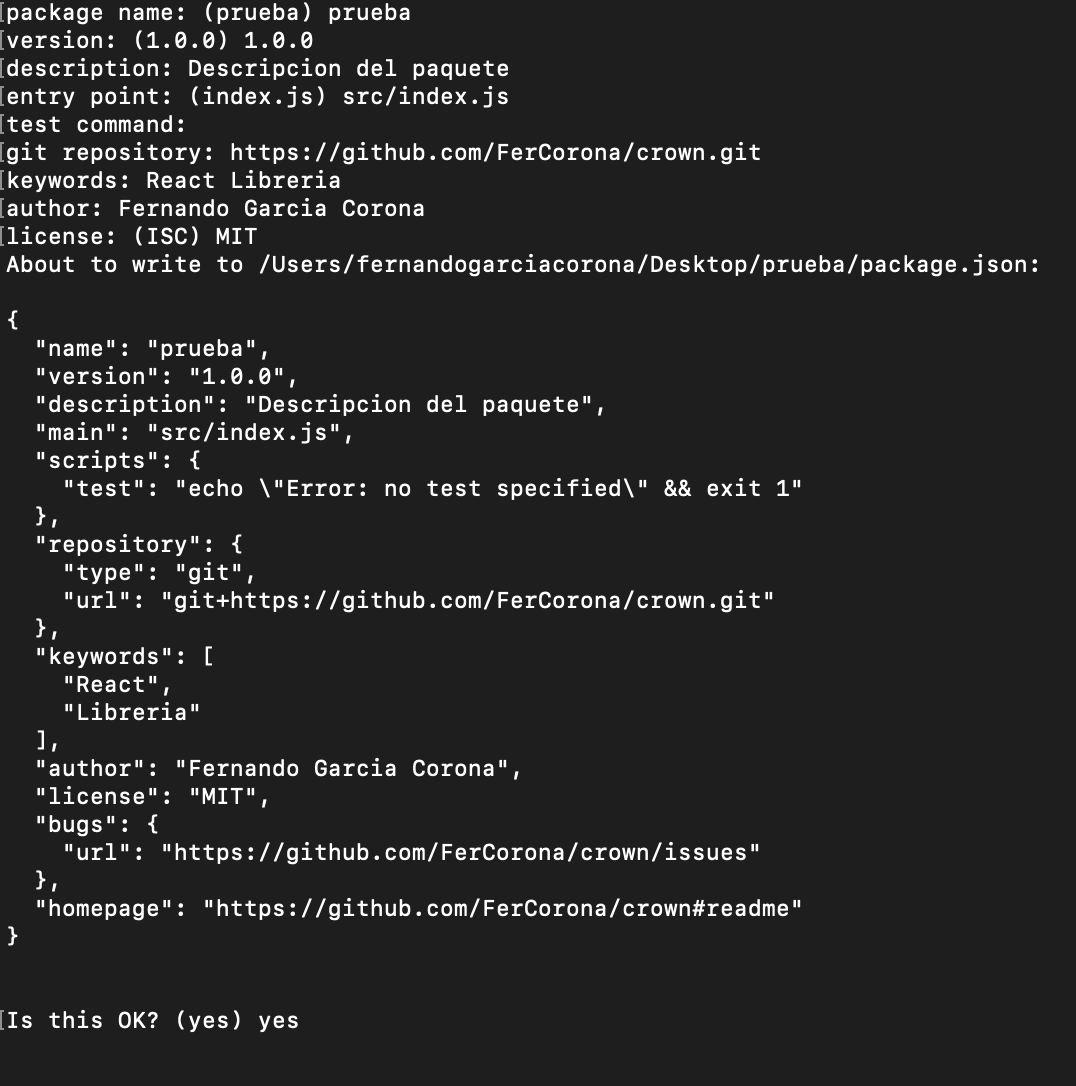
\includegraphics[width=1\textwidth]{./Imagenes/image9.png}
     \caption[Archivo de salida]{Archivo de salida}
         \end{figure}
    \newline
    \newline
    
    \subsection{Inicialización De Git En Nuestro Proyecto }
    Ahora se continuará agregando GIT en nuestro proyecto, esto nos garantizara el control de los cambios que se vayan realizando, para en caso de catástrofes poder regresar a una versión anterior, También podemos crear ramas,  para alojar nuevas funcionalidades que se requieran ser agregadas, eso sin afectar el estado del proyecto que ya está funcionando y cuando la nueva función esté completa y probada poder mezclarla con el original (la rama master).
    Incluir GIT no es una tarea compleja, basta con ejecutar el siguiente comando en la línea de comandos, esto dentro de nuestro directorio (“/Documents/crown”).
    \newline
    \newline
     \begin{figure}[H]
    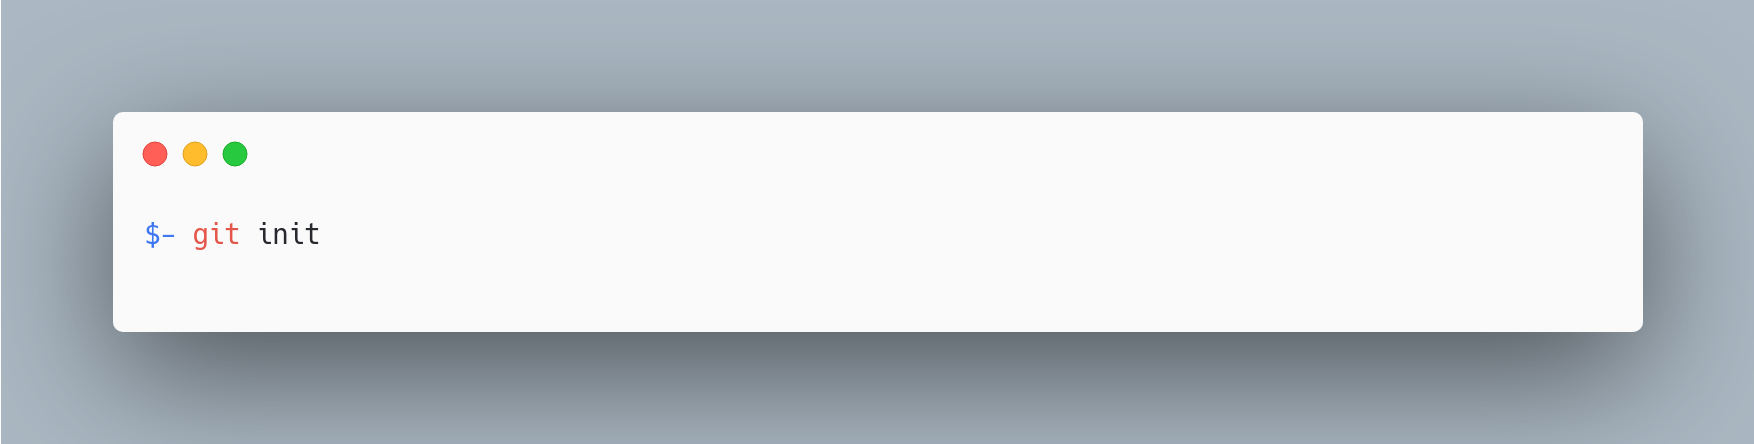
\includegraphics[width=1\textwidth]{./Imagenes/image35.png}
     \caption[Inicializar GIT]{Inicializar GIT}
         \end{figure}
    \newline
    \newline
    Creará una carpeta oculta (“/.git”) que nos permitirá manipular nuestro código con la línea de comandos de git, como crear ramas, hacer commit, hacer el merge de una rama etc.
    Para que esto funcione es necesario que el archivo creado anteriormente “package.json” conozca la ubicación remota de nuestro repositorio, se creó una cuenta en GITHUB  y se agregó un repositorio, el cual debemos copiar la dirección url y pegarla en el archivo “package.json”,  en el apartado llamado “repository” , en la llave “url” como se muestra en la imagen.
    Al la url que acabamos de copiar agregamos el prefijo “git+” y el postfijo “.git”.
    \newline
    \newline
     \begin{figure}[H]
    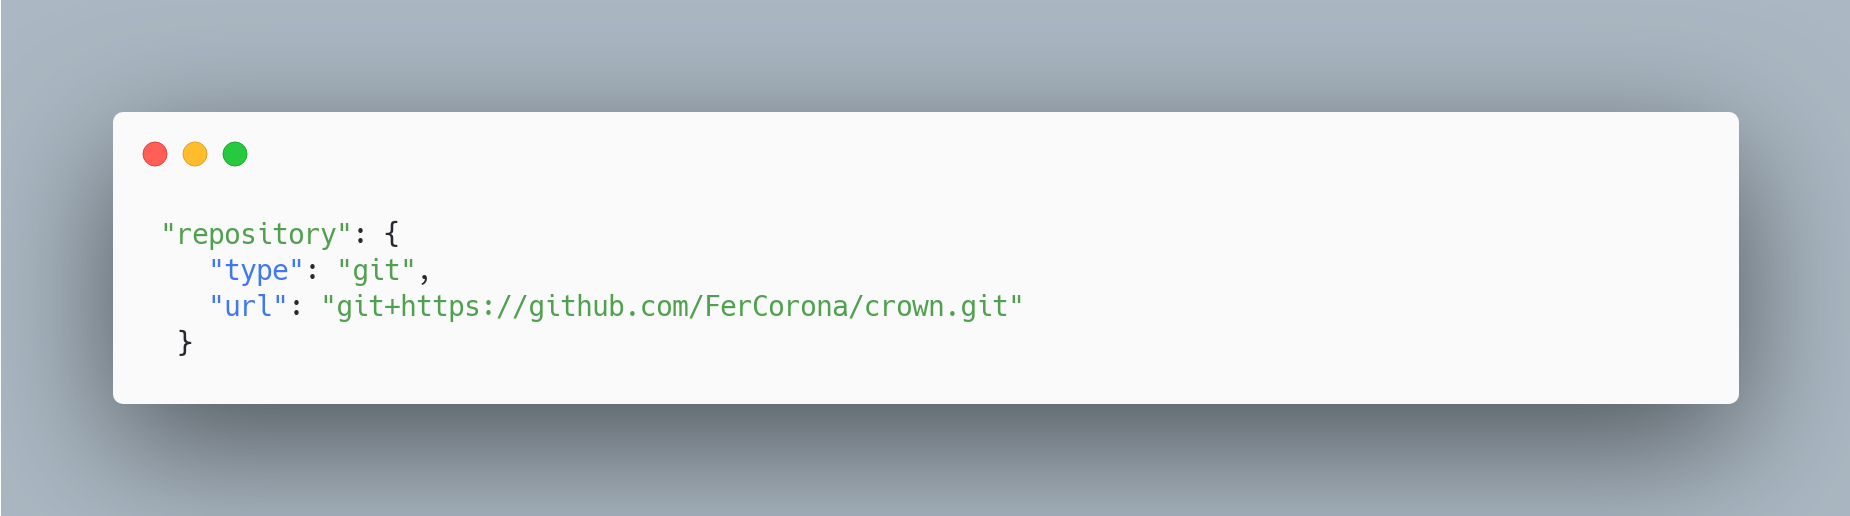
\includegraphics[width=1\textwidth]{./Imagenes/image4.png}
     \caption[Agregar repositorio existente]{Agregar repositorio existente}
         \end{figure}
    \newline
    \newline
    
    \subsection{Configuración Web-pack}
    Webpack es una tecnología utilizada en gran cantidad de proyectos de Front-end. Es útil cuando se trabaja en base a una estructura modular, en este caso modula nuestra librería para poder ser agregada en otros proyectos. Nos permite que el resultado final de nuestro proyecto sea menos pesado, esto es logrado por que concatena el código eliminando espacios no necesarios para el intérprete del navegador, lo que deja un archivo con código que no es del todo entendible para las personas pero que es muchos bits menos pesado para el navegador.
    También nos permite agregar cargadores para que pueda soportar SCSS, HTML JSX imágenes y otros archivos más.
    Para hacerlo funcionar debemos ejecutar una serie de comandos, que se enlistan a continuación, con ayuda de NPM.
    \newline
    \newline
     \begin{figure}[H]
    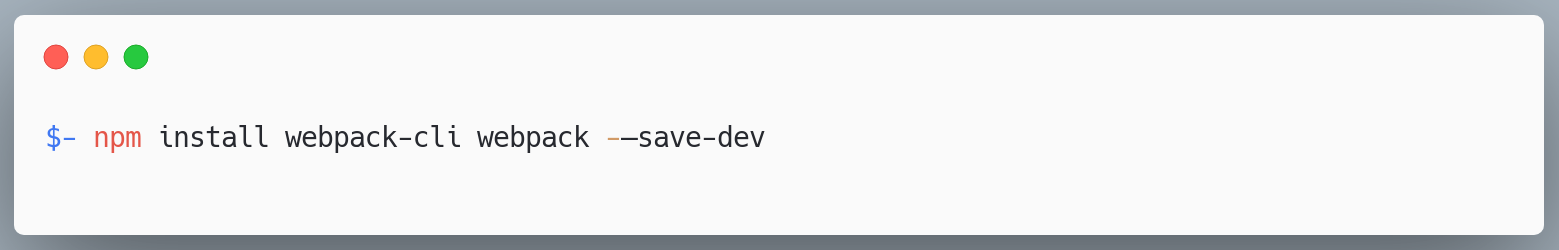
\includegraphics[width=1\textwidth]{./Imagenes/image3.png}
     \caption[Agregar Webpack]{Agregar Webpack}
         \end{figure}
    \newline
    \newline
    Los anteriores comandos agregan al proyecto en núcleo de Webpack, así como su cliente de comandos para la manipulación y visualización de archivos. Después de ejecutar los comandos se debe agregar los siguientes comandos en archivo “package.json”  en la sección de scripts, los script son los siguientes.
    \newline
    \newline
     \begin{figure}[H]
    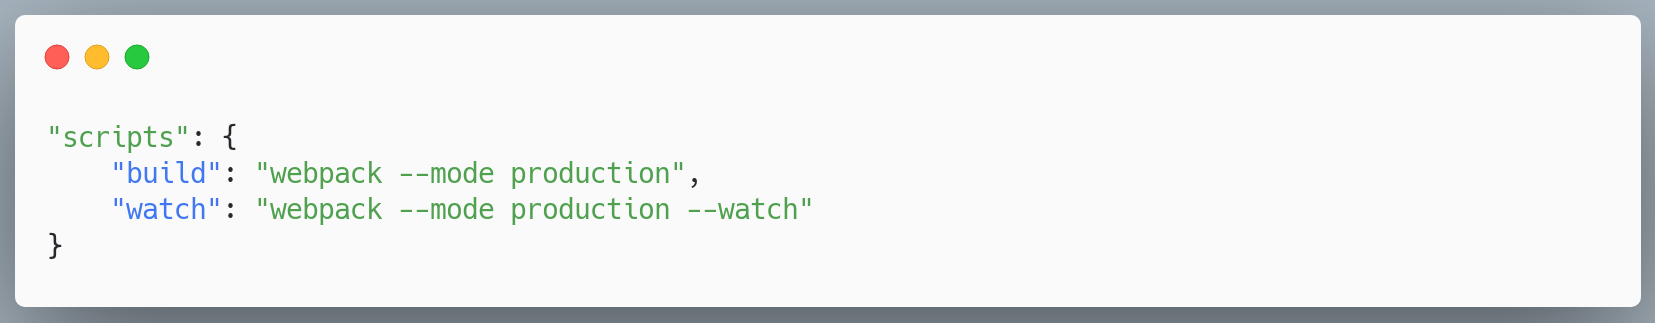
\includegraphics[width=1\textwidth]{./Imagenes/image6.png}
     \caption[Agregar scripts]{Agregar scripts}
         \end{figure}
    \newline
    \newline
    Los comandos agregados nos son de utilidad para:
    \begin{itemize}
    \item \textbf{Build:} Crear un archivo que estará listo para producción.
    \item \textbf{Watch:} Nos proporciona la misma funcionalidad que Build pero este, puede observar los cambios que estamos haciendo en tiempo real y actualizará el archivo final cada vez.
    \end{itemize}
    Para agregar configuración es necesario crear un archivo como se ilustra con el siguiente comando, estando en el directorio raíz de “crown”.
    \newline
    \newline
     \begin{figure}[H]
    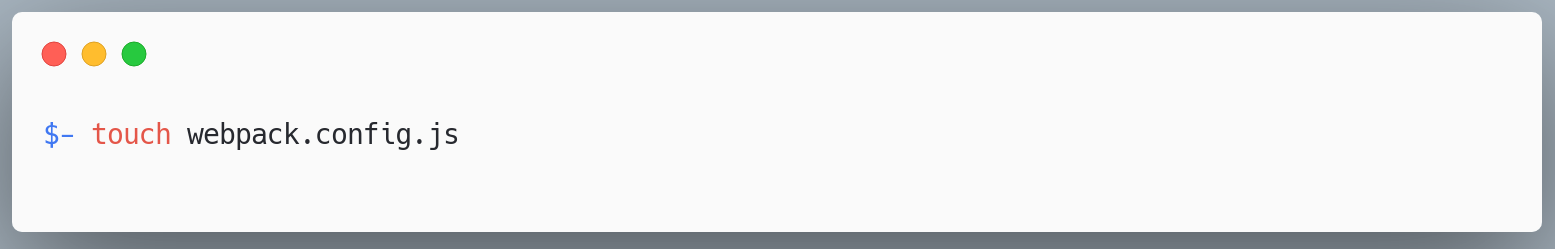
\includegraphics[width=1\textwidth]{./Imagenes/image38.png}
     \caption[Crear archivo vacío]{Crear archivo vacío}
         \end{figure}
    \newline
    Necesitamos agregar ciertos cargadores de Webpack para poder usar SASS y CSS, con el siguiente comando.
    \newline
    \newline
     \begin{figure}[H]
    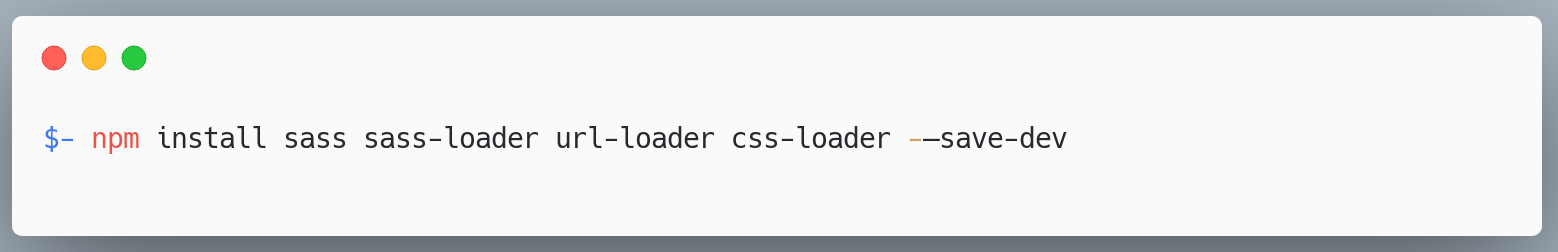
\includegraphics[width=1\textwidth]{./Imagenes/image8.png}
     \caption[Agregar cargadores de css]{Agregar cargadores de css}
         \end{figure}
    \newline
    \newline
    Con esto tenemos listas las dependencias necesarias para usar SASS / CSS y para poder manejar archivos como imágenes en JavaScript, tenemos que agregar la siguiente configuración en nuestro archivo Webpack.config.js.
    \newline
    \newline
     \begin{figure}[H]
    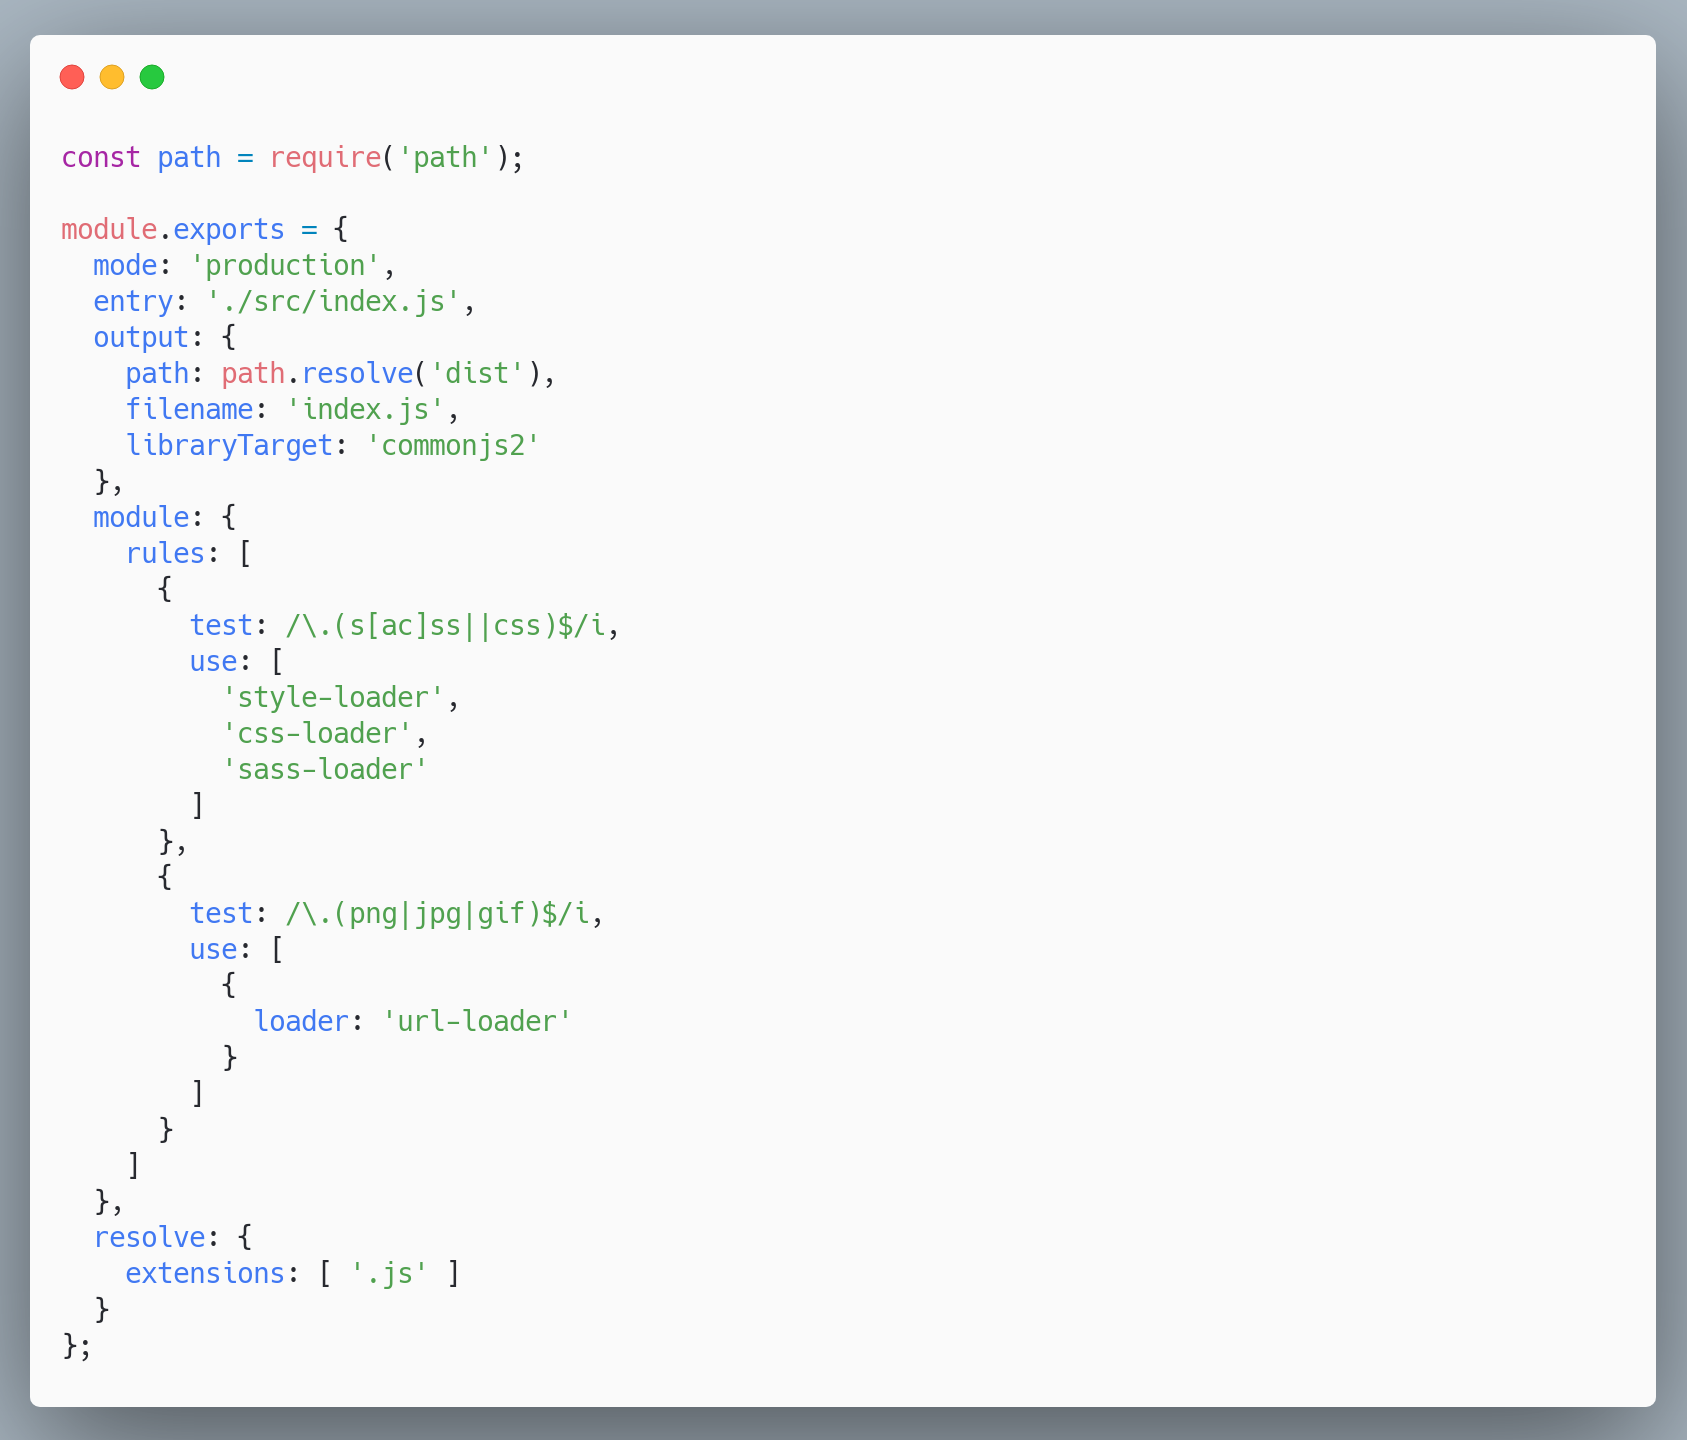
\includegraphics[width=1\textwidth]{./Imagenes/image2.png}
     \caption[Archivo final]{Archivo final}
         \end{figure}
    \newline
    La anterior configuración muestra cómo debe procesar cada tipo de archivo que encuentre dentro de nuestro proyecto, por eso dada una expresión regular que define extensiones de archivos puede usar un cargador a usar.
    Lo que es definido en la configuración es:
    \begin{itemize}
    \item \textbf{Entry: } Es el archivo inicial sobre el cual empezará el análisis del código si este tiene un import de otro archivo continuará sobre ese, esto generará un árbol. El directorio /src/index.js fue el dado para este caso.
    \item \textbf{Output: } Es el archivo en el que quedará la salida de nuestra librería en la dirección /dist/index.js
    \item \textbf{Rules: }Está incluido dentro de los módulos, esto agrega la manera en cómo se procesarán los archivos SCSS y CSS  con las dependencias style-loader, css-loader, sass-loader y por otra parte las imágenes con url-loader.
    \end{itemize}
    
    
    \subsection{Configuración Babel}
    Babel es un traductor de código JavaScript que permite convertir código de nuevas generaciones como el ES6 a versiones antiguas, extendiendo la compatibilidad a navegadores más viejos como Internet Explorer.
    Solo es necesario agregar las siguientes dependencias, con el siguiente comando.
    \newline
    \newline
     \begin{figure}[H]
    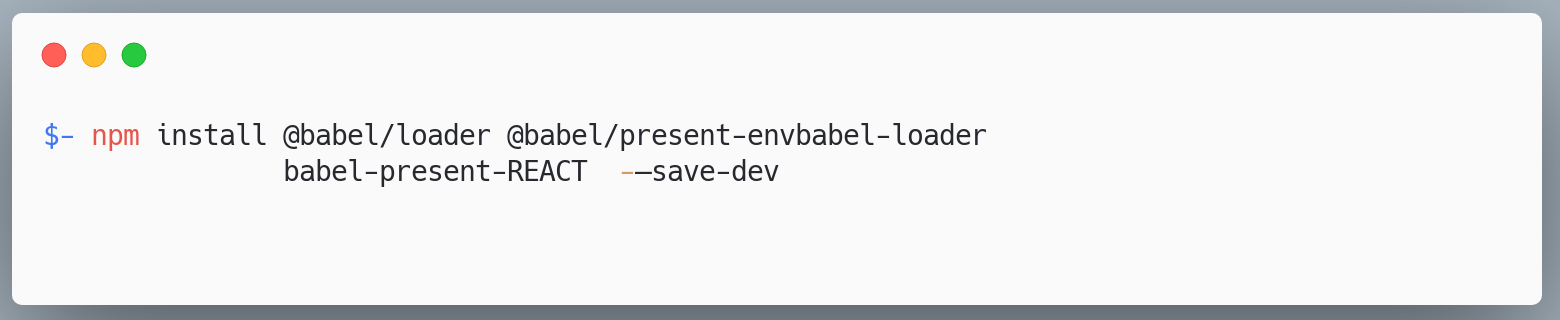
\includegraphics[width=1\textwidth]{./Imagenes/image36.png}
     \caption[Archivo Babel]{Archivo Babel}
         \end{figure}
    \newline
    \newline
    Después debemos crear un archivo en el directorio raíz llamado “.Babelrc”, al cual debemos agregar la siguiente configuración.
    \newline
    \newline
     \begin{figure}[H]
    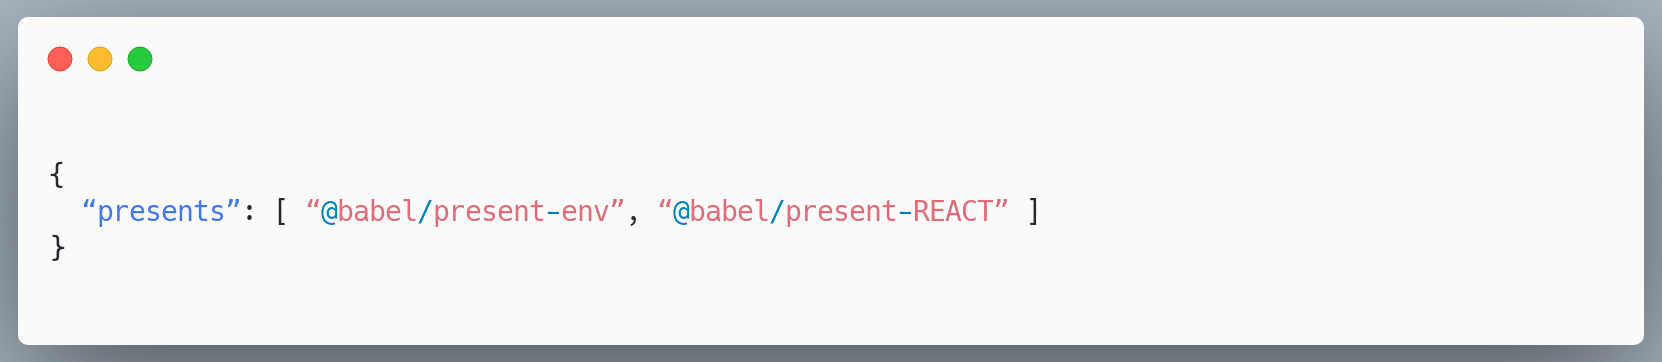
\includegraphics[width=1\textwidth]{./Imagenes/image17.png}
    \caption[Configurar Babel]{Configurar Babel}
    \end{figure}
    \newline
    \newline
    Y finalmente solo debemos agregar la siguiente configuración al archivo Webpack.config.js en el apartado de “rules” dentro de “module”.
    \newline
    \newline
     \begin{figure}[H]
    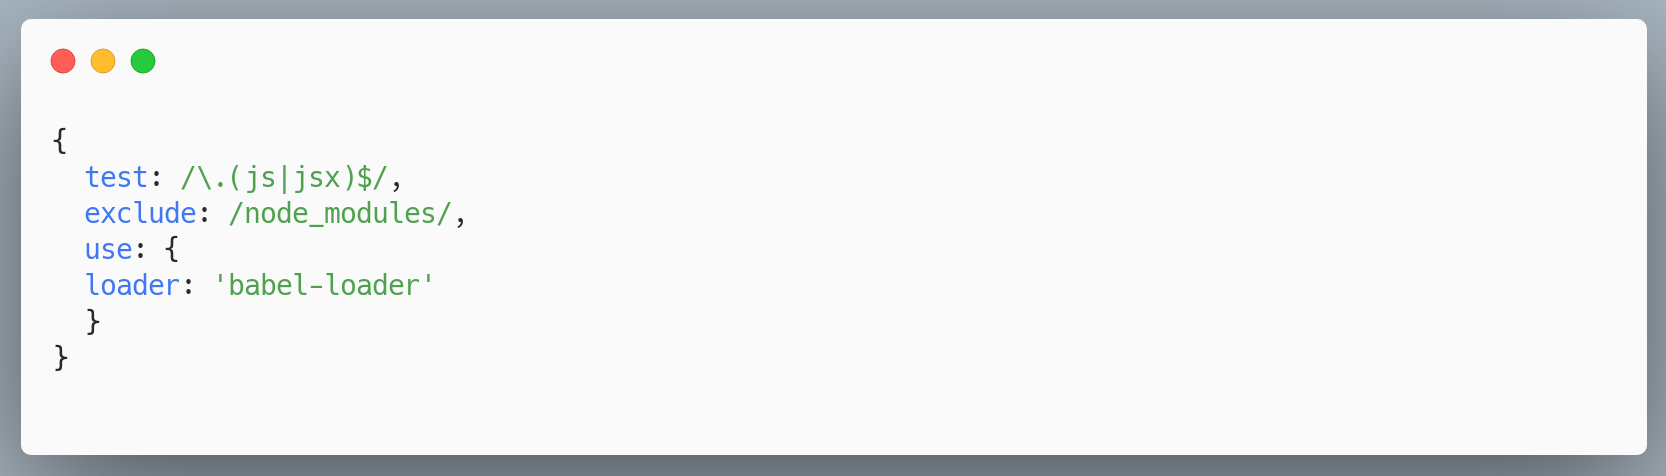
\includegraphics[width=1\textwidth]{./Imagenes/image1.png}
    \caption[Agregar Babel en Webpack]{Agregar Babel en Webpack}
    \end{figure}
    \newline
    \newline
    Esto para que WEWPACK sea el encargado de traducir el código con ayuda de Babel.
    
    
    \subsection{Agregar React Al Proyecto}
    React es una parte fundamental en el desarrollo de la presente librería y para agregarlo es necesario ejecutar el siguiente comando.
    \newline
    \newline
     \begin{figure}[H]
    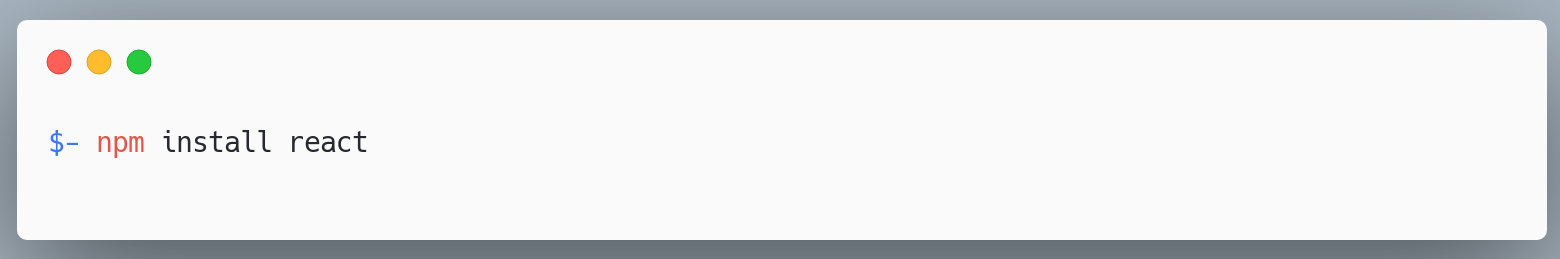
\includegraphics[width=1\textwidth]{./Imagenes/image23.png}
    \caption[Agregar React]{Agregar React}
    \end{figure}
    \newline
    \newline
    Para este comando no se agrega la bandera “–save-dev” al final, por que de esta manera forzamos a que cuando se instale esta librería también se instale React en caso de que no estuviera, ya que nuestra librería necesita React para su ejecución.
    
    
    \subsection{Configuración ESLint }
    Finalmente, para que nuestro espacio de desarrollo quede listo agregaremos ESLint que es un verificador de sintaxis, para tener un código limpio, con una clara indentación. Para que en toda la librería tengamos un código unificado. De igual manera no tendremos que preocuparnos por esto si no que al guardar el archivo obtenga el formato correcto.
    Para esto debemos ejecutar las siguientes dependencias en la terminal.
    \newline
    \newline
     \begin{figure}[H]
    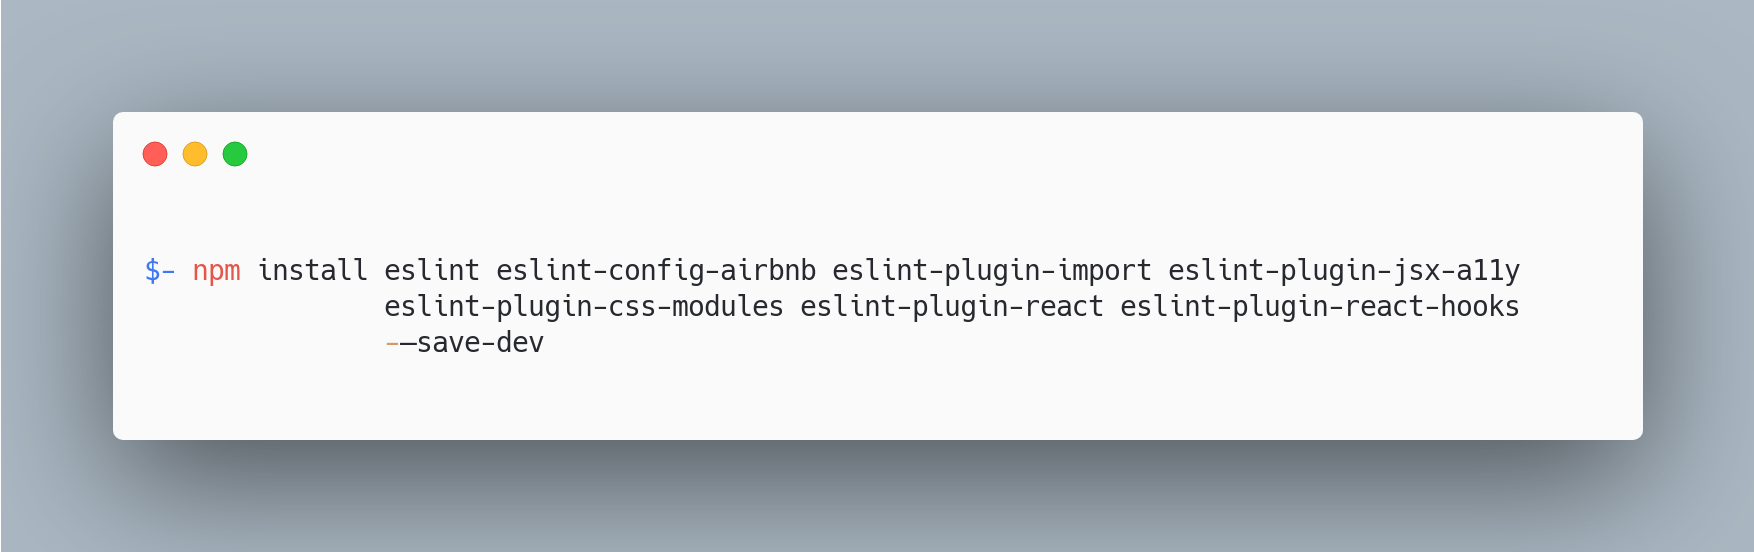
\includegraphics[width=1\textwidth]{./Imagenes/image14.png}
    \caption[Agregar ESLint]{Agregar ESLint}
    \end{figure}
    \newline
    \newline
    Dentro de las dependencias que agregamos se encuentran algunos complementos (plugins) que nos ayudan a dar formato a los archivos JSX, a verificar la sintaxis de React y  puede verificar que la importación de algún archivo realmente arroje un resultado.
    Debemos agregar un archivo en el que definiremos un conjunto de reglas específicas las cuales nuestros archivos van a cumplir, para agregar el archivo se debe ejecutar el siguiente comando.
    \newline
    \newline
     \begin{figure}[H]
    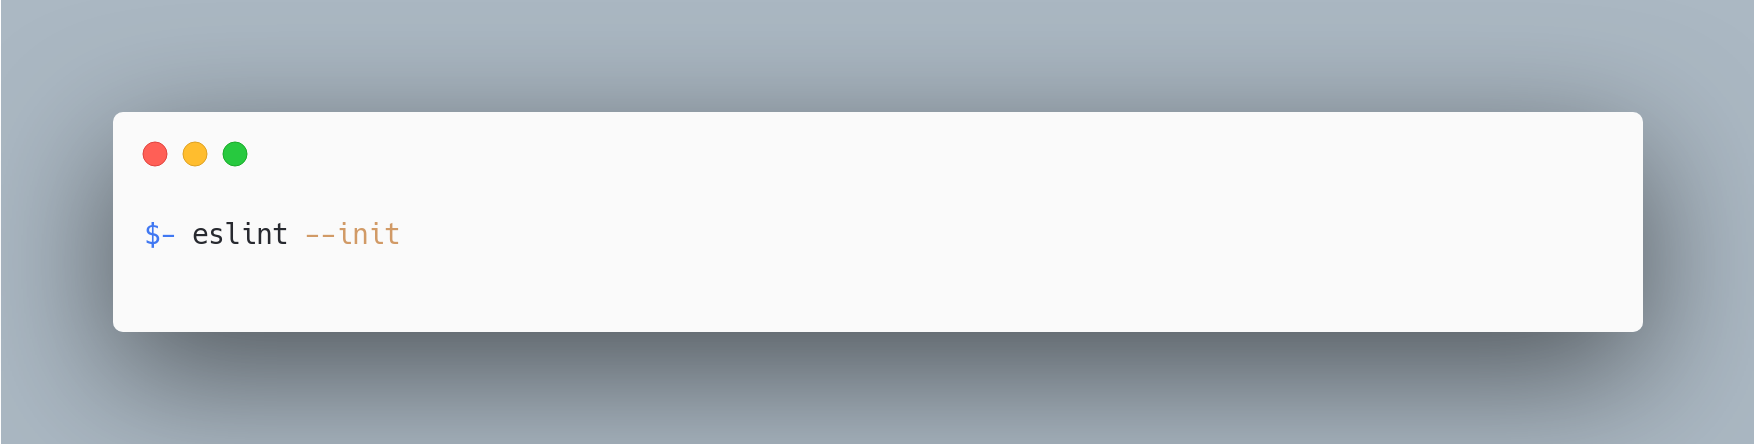
\includegraphics[width=1\textwidth]{./Imagenes/image32.png}
    \caption[Inicializar ESLint]{Inicializar ESLint}
    \end{figure}
    \newline
    \newline
    Después de ejecutar el comando este preguntara por datos para la configuración de ESLint, a continuación, se enlistan cada uno de los datos introducidos.
    \begin{itemize}
    \item \textbf{Uso de ESLint:  }Seleccionaremos el uso que le daremos a ESLint, que en este caso es checar sintaxis, encontrar problemas y forzar el estilo del código.
    \item \textbf{Tipo de módulos que usa el proyecto:} Seleccionaremos la opción JavaScript modules, por que es el tipo de importaciones y exportaciones que estaremos usando.
    \item \textbf{Framework por usar: }Seleccionaremos React.
    \item ¿Se usará TYPESCRIPT?: Se selecciona no. 
    \item ¿Donde se ejecutará?: Debemos seleccionar navegador.
    \item \textbf{Guía de estilos que se usará en el proyecto: } Nosotros elegiremos usar una guía popular  y después escogemos Airbnb.
    \item Formato del archivo de salida: Nosotros debemos escoger JavaScript.
    \end{itemize}
    Con esto tenemos todo listo para comenzar con el desarrollo de nuestra librería.
    \newpage

				
			\section {Lineamientos UX/UI}
				Uno de los puntos clave para obtener los resultados esperados de la biblioteca, es tomar en cuenta la experiencia de usuario ( UX ) y la interfaz de usuario ( UI ), que podrían definirse de la siguiente manera.

\begin{itemize}
\item \textbf{Experiencia de usuario ( UX ): } Es la sensación que una persona percibe, al usar una herramienta como puede ser una página web, o aplicación móvil, esto incluye la funcionalidad y la respuesta que recibe, logrando que una persona sienta que ya conoce la aplicación y conocer cada acción que realiza.
\item \textbf{Interfaz de usuario ( UI ):  } Es la percepción visual de una web o aplicación móvil, esta puede ser agradable para el usuario y generar el interés o rechazo de la misma, y llegar a sentir emociones.
\end{itemize}

Se han encontrado una serie de parámetros, los cuales se logran obtener una interfaz y experiencia de usuario favorables, que serán implementados en la presente biblioteca.

\begin{itemize}
\item \textbf{Sombras:} El uso de las sombras en los elementos de una interfaz gráfica, genera un mayor interés entre los elementos mostrados y da el efecto de tener una mayor altura dimensional.
\item \textbf{Jerarquía de elementos:} Para que el usuario entienda el objetivo de la aplicación Web debe existir una jerarquía visual, para que el usuario entienda cual es el objetivo de la Web representado por elementos visualmente más grandes y los elementos por los cuales no tendrían que tener tanta importancia serán más pequeños.
\item \textbf{Alineación vertical y horizontal:} Este punto puede ser visto como generar una cuadrícula, la cual cada elemento coincide vertical y horizontalmente.
\item \textbf{Retroalimentación:} Para que el usuario tenga la sensación de que tiene todo el control de la Web y que sienta que sabe que está haciendo siempre, se deben proporcionar efectos para que esto sea posible, por ejemplo cuando pasas el mouse sobre algún elemento este debe reaccionar.
\item \textbf{Tipo de fuente:} Para la correcta legibilidad de cualquier texto en la biblioteca se usará la fuente llamada San Francisco desarrollada por Apple de la familia de las fuentes Sans-Serif.
\item \textbf{Alto de línea:} Si se aumenta el alto de la línea permitirá que en un texto sea más legible porque existirá más espacio y no se tendrá texto que parezca encimado.
\item \textbf{Consistencia:} Este punto trata de que todos los elementos tengan similitudes entre sí, no importa si sean del mismo tipo, esto será fácil para que el usuario conozca cada una de las pantallas aunque sea la primera vez que se visita. 
\item \textbf{Colores:} Existe una actual tendencia por el uso de colores pasteles, ya que estos te hacen sentir familiar, ya que estos están presentes mayormente en la naturaleza.
\end{itemize}

				
			\section {Desarrollo}
				\subsection{Configuración Archivo Inicial}
El proyecto contendrá un nodo raíz el cual será el que tendrá los llamados al conjunto de elementos que tendrá nuestra librería. Anteriormente se creó un directorio llamado “src” en la raíz de “crown”, dentro de “src” debemos crear un archivo llamado “index.js” este es un archivo de JavaScript el cual definiremos como punto de inicio de Webpack  y a partir de este buscará todas las importaciones de otros submódulos. Con el siguiente comando creamos el archivo requerido.
\newline
\newline
     \begin{figure}[H]
    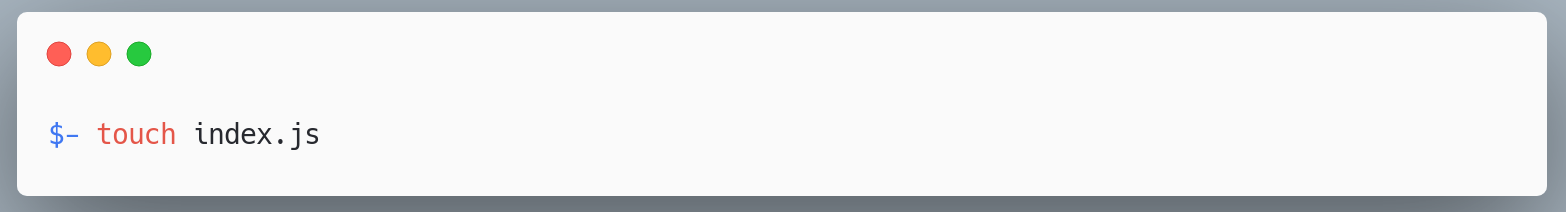
\includegraphics[width=1\textwidth]{./Imagenes/carbon.png}
    \caption[Inicializar archivo vacío]{Inicializar archivo vacío}
    \end{figure}
\newline
\newline
Dentro de este archivo debemos poner el llamado a cada elemento que se vaya agregando a nuestra librería ( Botones, Campos de texto, Tablas etc.), en la siguiente ilustración se muestra la manera en que se deben agregar los elementos.
\newline
\newline
\begin{figure}[H]
    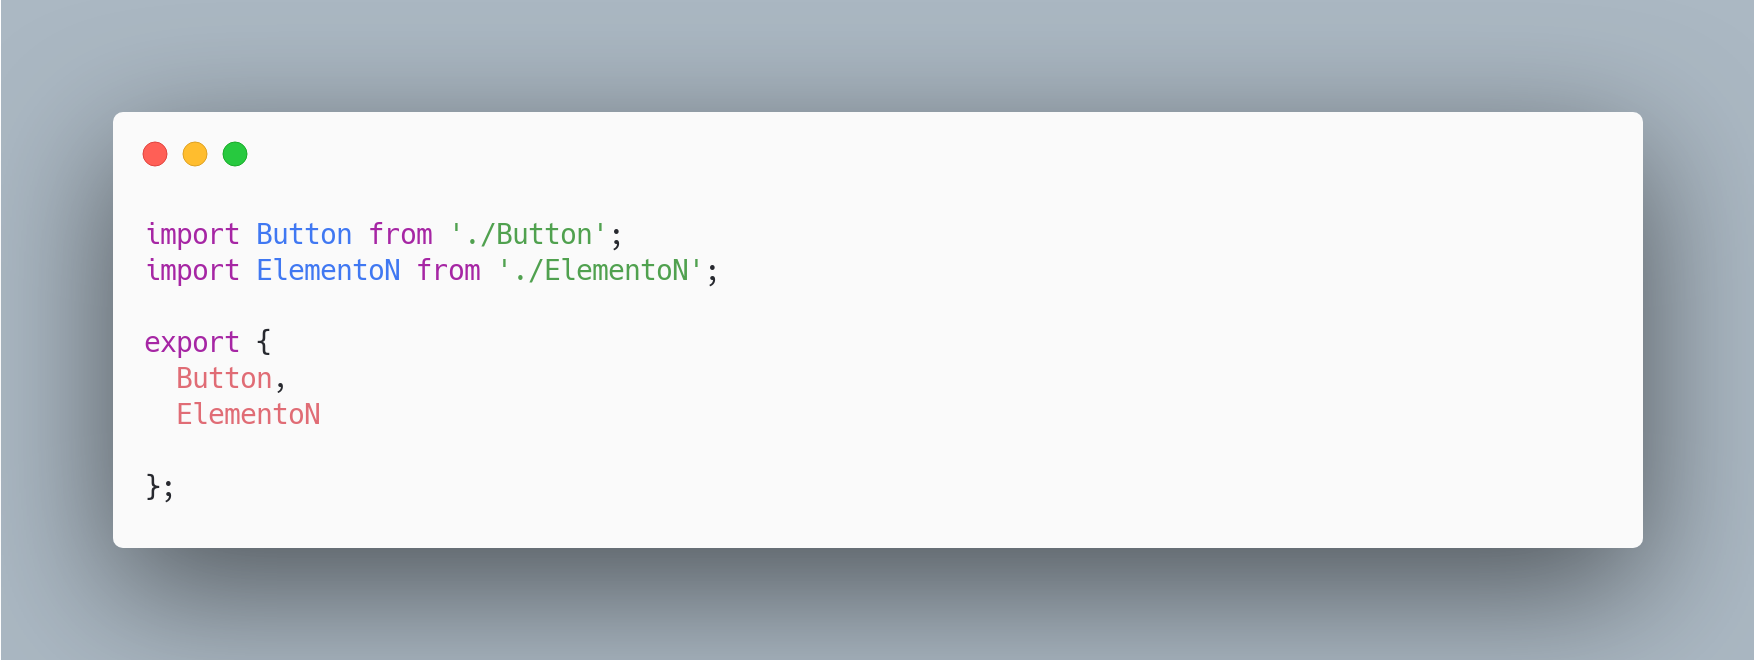
\includegraphics[width=1\textwidth]{./Imagenes/carbon-2.png}
    \caption[Inclusión de los elementos]{Inclusión de los elementos}
    \end{figure}
\newline
\newline
El primer bloque de código muestra la importación de cada uno de los elementos a nuestro archivo index, y la segunda parte exportamos un objeto de JAVASCRIPT con cada uno de los elementos.
Webpack analiza cada elemento que se incluye en el objeto y busca el contenido existente dentro de cada uno.
Cada uno de los elementos que se necesita agregar deben estar situados a la misma altura del archivo “index.js” esto dentro del directorio “src” para que puedan ser procesados.



\subsection{Elemento Botón}
El primer elemento que vamos a agregar es el botón, para esto creamos un directorio llamado “Botton” de la siguiente manera.
\newline
\newline
\begin{figure}[H]
    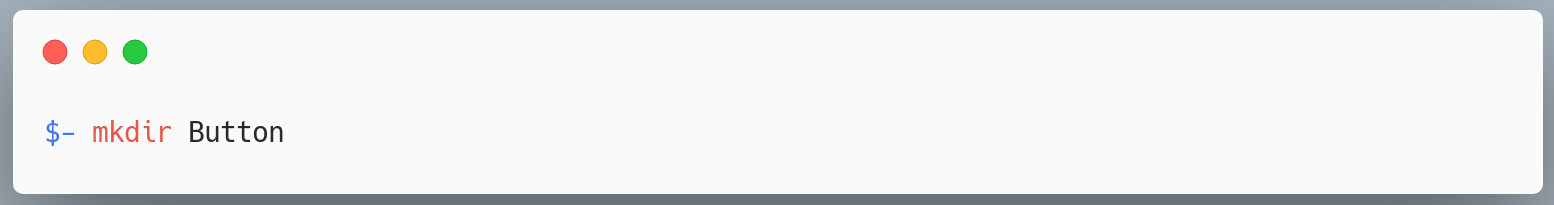
\includegraphics[width=1\textwidth]{./Imagenes/carbon-3.png}
    \caption[Crear directorio para el elemento Button]{Crear directorio para el elemento Button}
    \end{figure}
\newline
\newline
Y dentro de este directorio crearemos dos archivo que son los que incluirán el núcleo de nuestro botón, el primer archivo se llamará “index.js ” esto es así ya que por defecto, cuando importas un archivo que está dentro de un directorio, JAVASCRIPT toma el que es llamado “index.js” y no es necesario especificar este dato, esto lo podemos ver de manera clara en el archivo inicial “index.js” que está al mismo nivel que el directorio “Botton”, el cual importa el elemento Botton pero no especifica el archivo. Este archivo solamente hace el llamado al segundo archivo “Botton.js” que es el que tiene el código fuente del botón. 
\newline
\newline
\begin{figure}[H]
    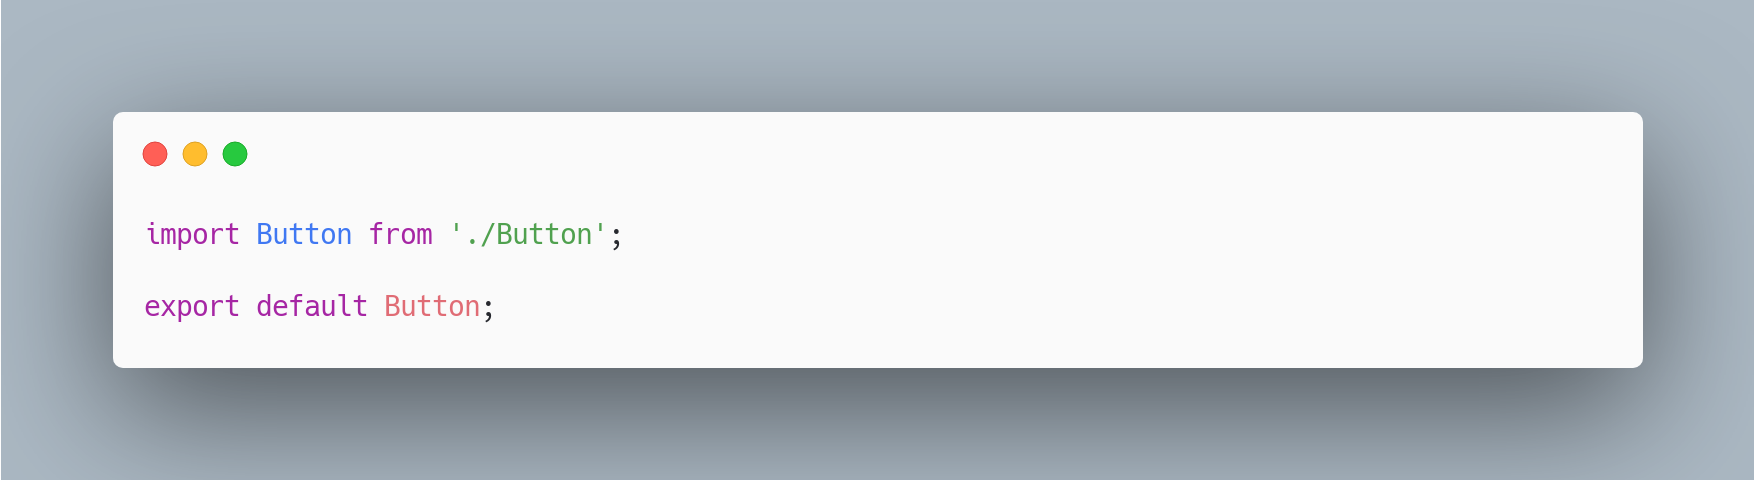
\includegraphics[width=1\textwidth]{./Imagenes/carbon-5.png}
    \caption[Contenido del elemento Button]{Contenido del elemento Button}
    \end{figure}
\newline
\newline
El segundo archivo ya mencionado “Botton.js”  hace el render de nuestro botón, y gestiona la configuración que el usuario final quiera asignarle.
En la siguiente tabla se muestran los props ( configuración inicial  ) del botón.
\newline
\newline
\begin{center}
 \begin{tabular}{ | c |  p{5cm}  | c | p{3cm} |} 
 \hline
 \textbf{Nombre} &  \textbf{Uso} &  \textbf{ Tipo de dato} &  \textbf{Valor por defecto}\\ [0.5ex] 
 \hline\hline
text & Texto que mostrará el botón.  &  Cadena de texto. & Click me! \\  [2.5ex] 
 \hline
onClick & Es la función que ejecutará cuando se hace click. & Funcion. & Función vacía. \\[2.5ex] 
 \hline
color &  Es el color del botón. & Cadena de texto. & --blue-4 \\[3.5ex] 
 \hline
 textColor & Es el color del texto en el botón. &  Cadena de texto. & --white \\[2.5ex] 
 \hline
borderColor & Es el color del borde del botón. & Cadena de texto. & --blue-4 \\ [2.5ex] 
 \hline
 type & Es el tipo de botón. & Cadena de texto. & Default \\ [2.5ex] 
 \hline
 shape & Es la forma del botón. Estos valores agregaran una curvatura, tenemos Round y SemiRound uno mas curvo que otro. & Cadena de texto. & Round \\ [2.5ex] 
 \hline
 shadow & Especifica si el botón debe tener una sombra. & Cadena de texto. & Booleano. \\ [2.5ex] 
 \hline
\end{tabular}
\end{center}
\newline
\newline
\newline
Los tipos (type) de botones que podemos tener son los siguientes.
\begin{itemize}
\item \textbf{Default:} Es el botón que se recomienda usar como principal.
\item \textbf{Secondary:} Es recomendable usarlo si ya se usa un botón default, para cuidar la jerarquía visual.
\item \textbf{Text:} Este es un botón sin contorno, debe ser usado para acciones con poca importancia.
\end{itemize}
Los colores que se usan son una constante definida por la librería ya que se considera que son cromáticamente compatibles entre ellos, este tema se abordará más adelante.
A continuación se muestra un fragmento del código que permite agregar la configuración requerida.
\newline
\newline
\begin{figure}[H]
    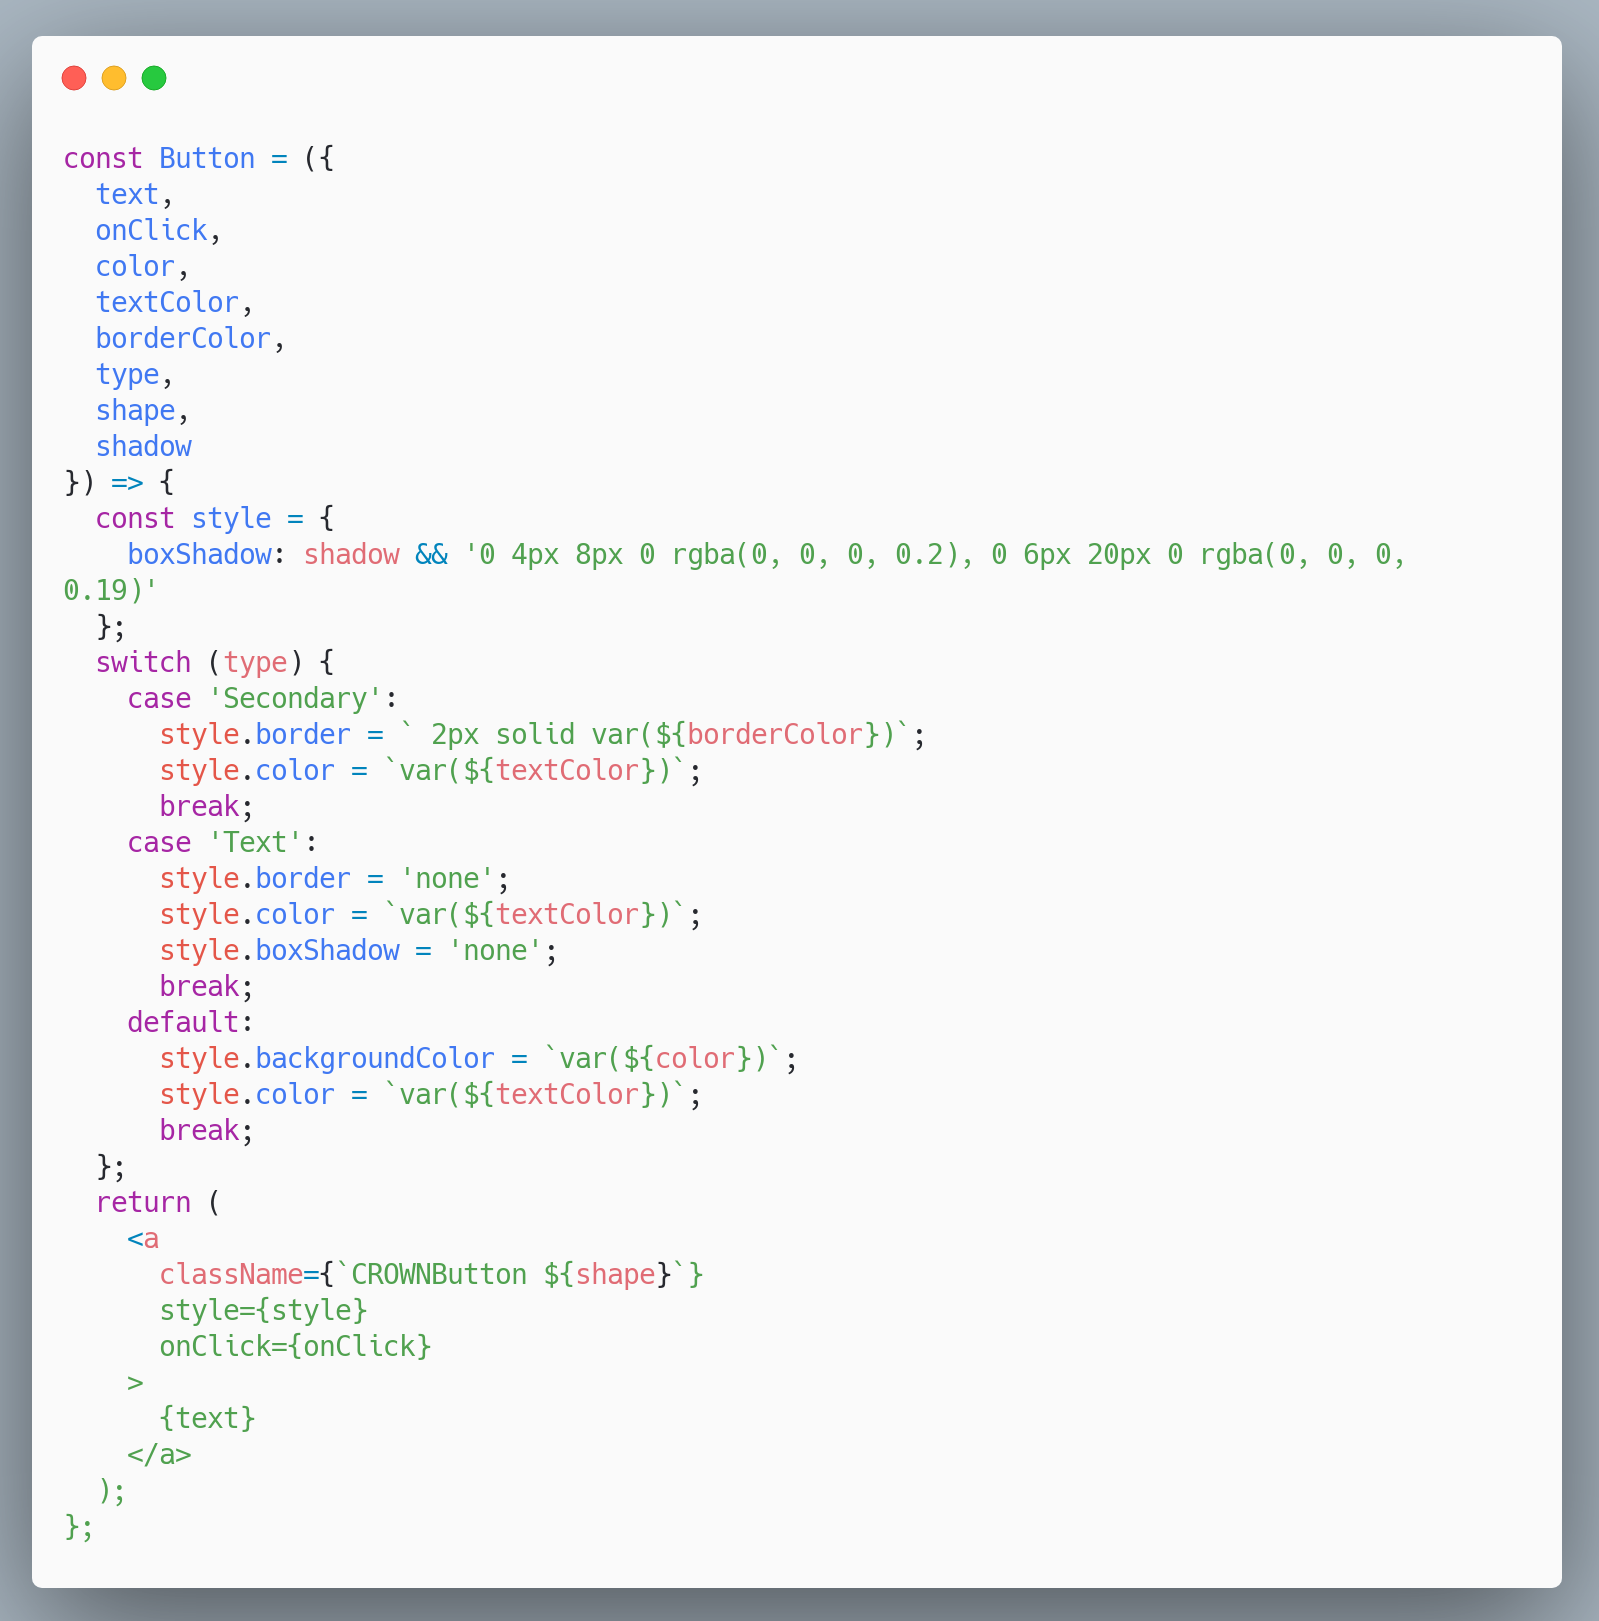
\includegraphics[width=1\textwidth]{./Imagenes/carbon-9.png}
    \caption[Código fuente del elemento Button]{Código fuente del elemento Button}
    \end{figure}
\newline
\newline
En la primera parte podemos ver una lista de la configuración dada,  después definimos un objeto llamado styles el cual agrega dentro de un switch el CSS para que sea mostrado de acuerdo al tipo ( type ) de botón que se quiere. Finalmente regresa HTML el cual es nuestro botón configurado.
Se puede observar que dentro de la etiqueta <a> tenemos “className” esto agrega la clase en la cual definiremos el CSS.
Dentro del archivo CSS agregamos el diseño base de nuestro botón, aquí tenemos el  tamaño de la letra, tamaño del botón, grosor de letra y otras cosas más.
\newline
\newline
\begin{figure}[H]
    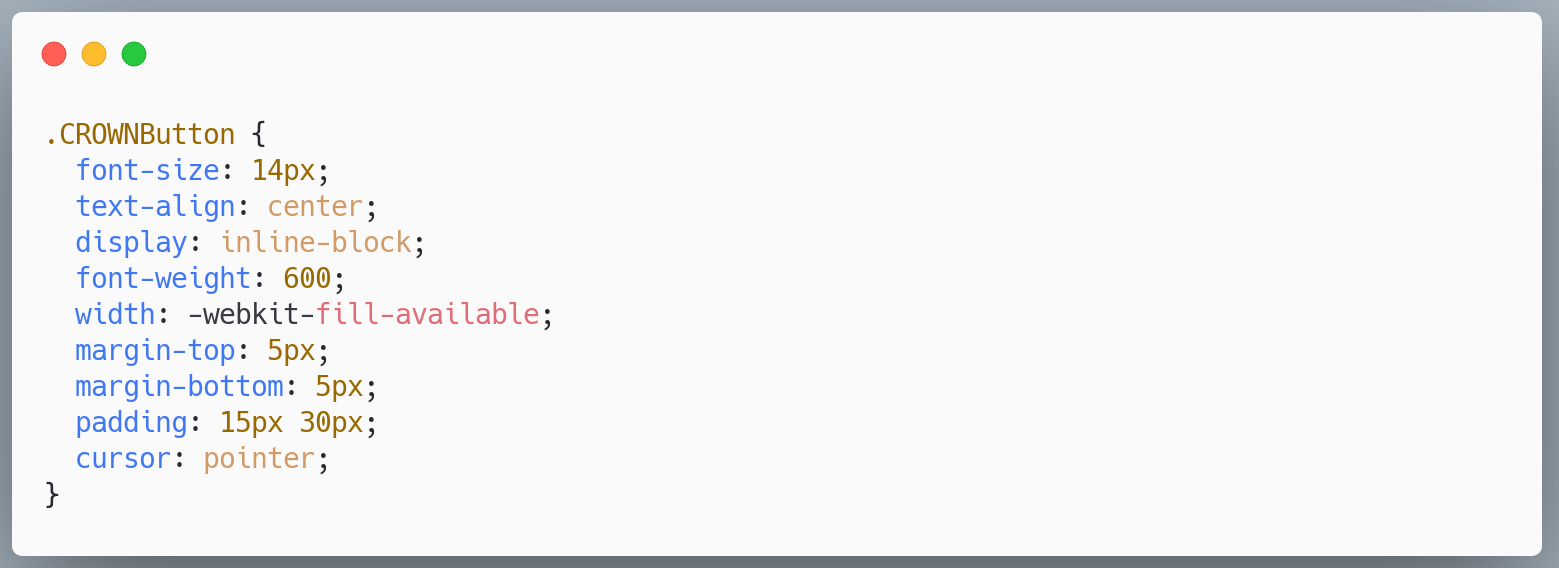
\includegraphics[width=1\textwidth]{./Imagenes/image26.png}
    \caption[Estilos del elemento Button]{Estilos del elemento Button}
    \end{figure}
\newline
\newline



\subsection{Elemento Label}
Ahora vamos a agregar el elemento Label que es un texto con el cual tenemos un formato estandarizado para tener un mejor diseño. En este elemento podemos dar parámetros de configuración como el tamaño, grosor y color que son los elementos básicos que se usan cuando estamos formateando con CSS nuestro texto. 
A continuación se presenta una lista de los parámetros y  su significado.
\newline
\begin{center}
 \begin{tabular}{ | c |  p{5cm}  | c | p{3cm} |} 
 \hline
 \textbf{Nombre} &  \textbf{Uso} &  \textbf{ Tipo de dato} &  \textbf{Valor por defecto}\\ [0.5ex] 
 \hline\hline
text 		& Este parámetro  indica el texto que vamos a mostrar.  &  Cadena de texto. 	& “I’m a label” \\  [2.5ex] 
 \hline
size 	        & Indicamos el tamaño del texto. Se cuenta con un conjunto de tamaños establecidos que se mencionan en el apartado de las constantes.       & Cadena de texto.  	& small \\[2.5ex] 
 \hline
color        & Es el color del texto.						    & Cadena de texto. 	& --black-0 \\[3.5ex] 
 \hline
 weight.   & Indicamos el grosor del texto. Se cuenta con un conjunto de tamaños establecidos que se mencionan en el apartado de las constantes.&  Cadena de texto. 	& regular \\[2.5ex] 
 \hline
\end{tabular}
\end{center}
\newline
\newline
Para el funcionamiento de la etiqueta de texto se tiene un componente de react en el cual se crea un objeto de JAVASCRIPT, se agrega la configuración del color, tamaño de texto y grosor. Finalmente se crea una etiqueta de HTML a la cual le damos nuestro objeto para que aplique el estilo y le ponemos el texto que se quiere mostrar.
\newline
\newline
\begin{figure}[H]
    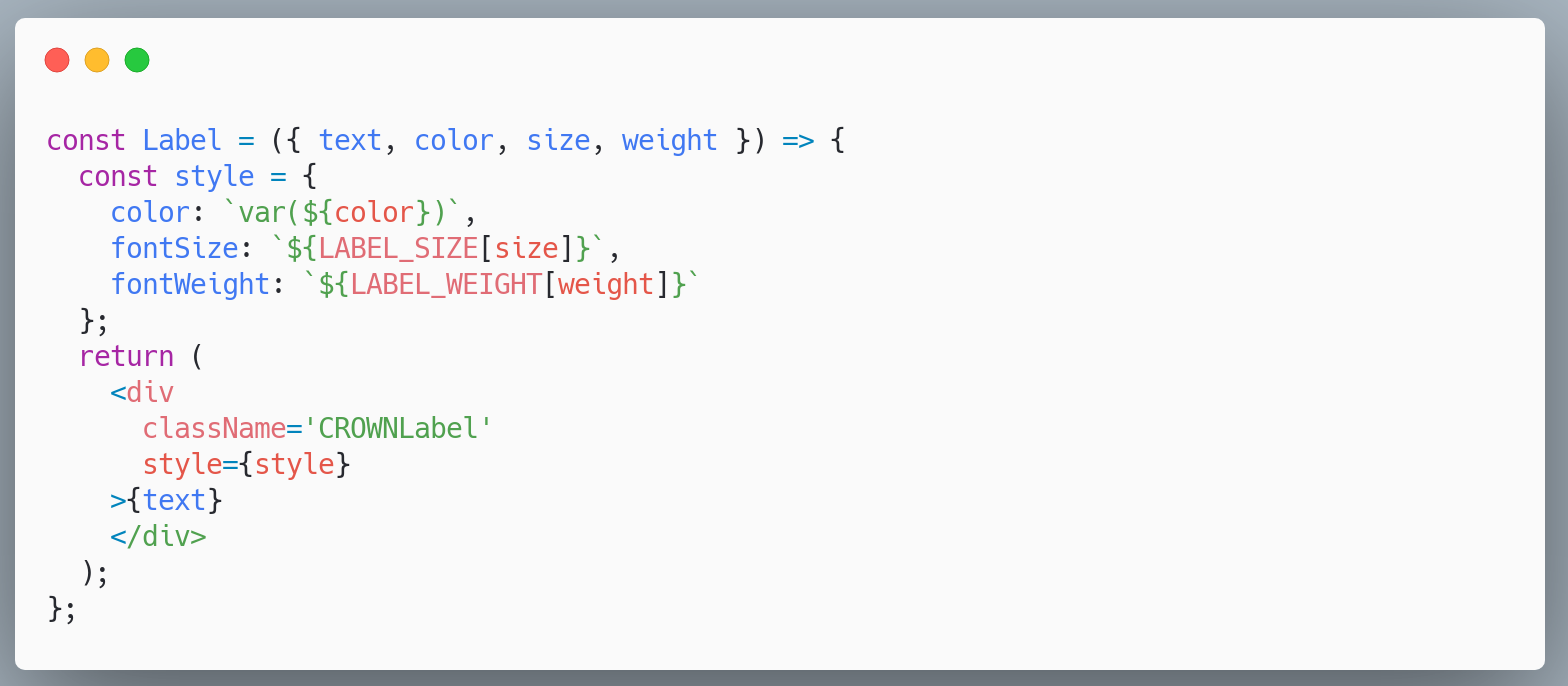
\includegraphics[width=1\textwidth]{./Imagenes/carbon-11.png}
    \caption[Código fuente del elemento Label]{Código fuente del elemento Label}
    \end{figure}
\newline
\newline



\subsection{Elemento Input Tex}
El input text es de utilidad para permitir la entrada de datos, y posteriormente puede ser procesado para enviarlos a algún servicio o procesarlos dentro de nuestra aplicación en donde es implementado.
Los datos de entrada que son necesarios para configurar el elemento se muestran a continuación.
\newline
\newline
\begin{center}
 \begin{tabular}{ | c |  p{5cm}  | c | p{3cm} |} 
 \hline
 \textbf{Nombre} &  \textbf{Uso} &  \textbf{ Tipo de dato} &  \textbf{Valor por defecto}\\ [0.5ex] 
 \hline\hline
placeholder &Es el texto que muestra el InputText si se desea poner.  &  Cadena de texto. 	& “Write on me!” \\  [2.5ex] 
 \hline
onChange & Es la función que va a hacer invocada cuando se escriba.     & Función vacía.  	& Función vacía.l \\[2.5ex] 
 \hline
nameState & Es el nombre con el cual se identifica en el estado.    & Cadena de texto.	& input \\[3.5ex] 
 \hline
 type   & Es la manera en como será interpretado por Input Text, estos son los que existen por defecto en HTML. Password etc.&  Cadena de texto.	& text \\[2.5ex] 
 \hline
 title  & Si se pone como “true” este agregara un Label antes del Input Text y no lo pondrá dentro.&  Booleano.	& false \\[2.5ex] 
 \hline
 extraStyle   & Si se desea agregar más estilos se puede poner el nombre de la clase CSS para poder ser manipulado.&  Cadena de texto. 	& Cadena vacía. \\[2.5ex] 
 \hline
\end{tabular}
\end{center}
\newline
\newline
La primera consideración que se tiene, es saber si se necesita tener un “Título” en nuestro Input Text, y si es así, se agrega un elemento Label antes,  para mostrar cual es el significado de nuestro label. Esto por ejemplo, si se quiere poner una entrada de texto para solicitar el correo electronico de cierta persona, esto puede estar dentro de el Input Texto denominado placeholder o afuera denominado title, por defecto title está desactivado y se activa enviando “true”.
Cuando se escribe sobre el campo de texto, este llama a la función “onChange” que recibe, se regresa el nombre de como está identificado en el estado de REACT y el valor que contiene el campo de texto.
Los demás parámetros de los estilos también son agregados en el siguiente código.
\newline
\newline
\begin{figure}[H]
    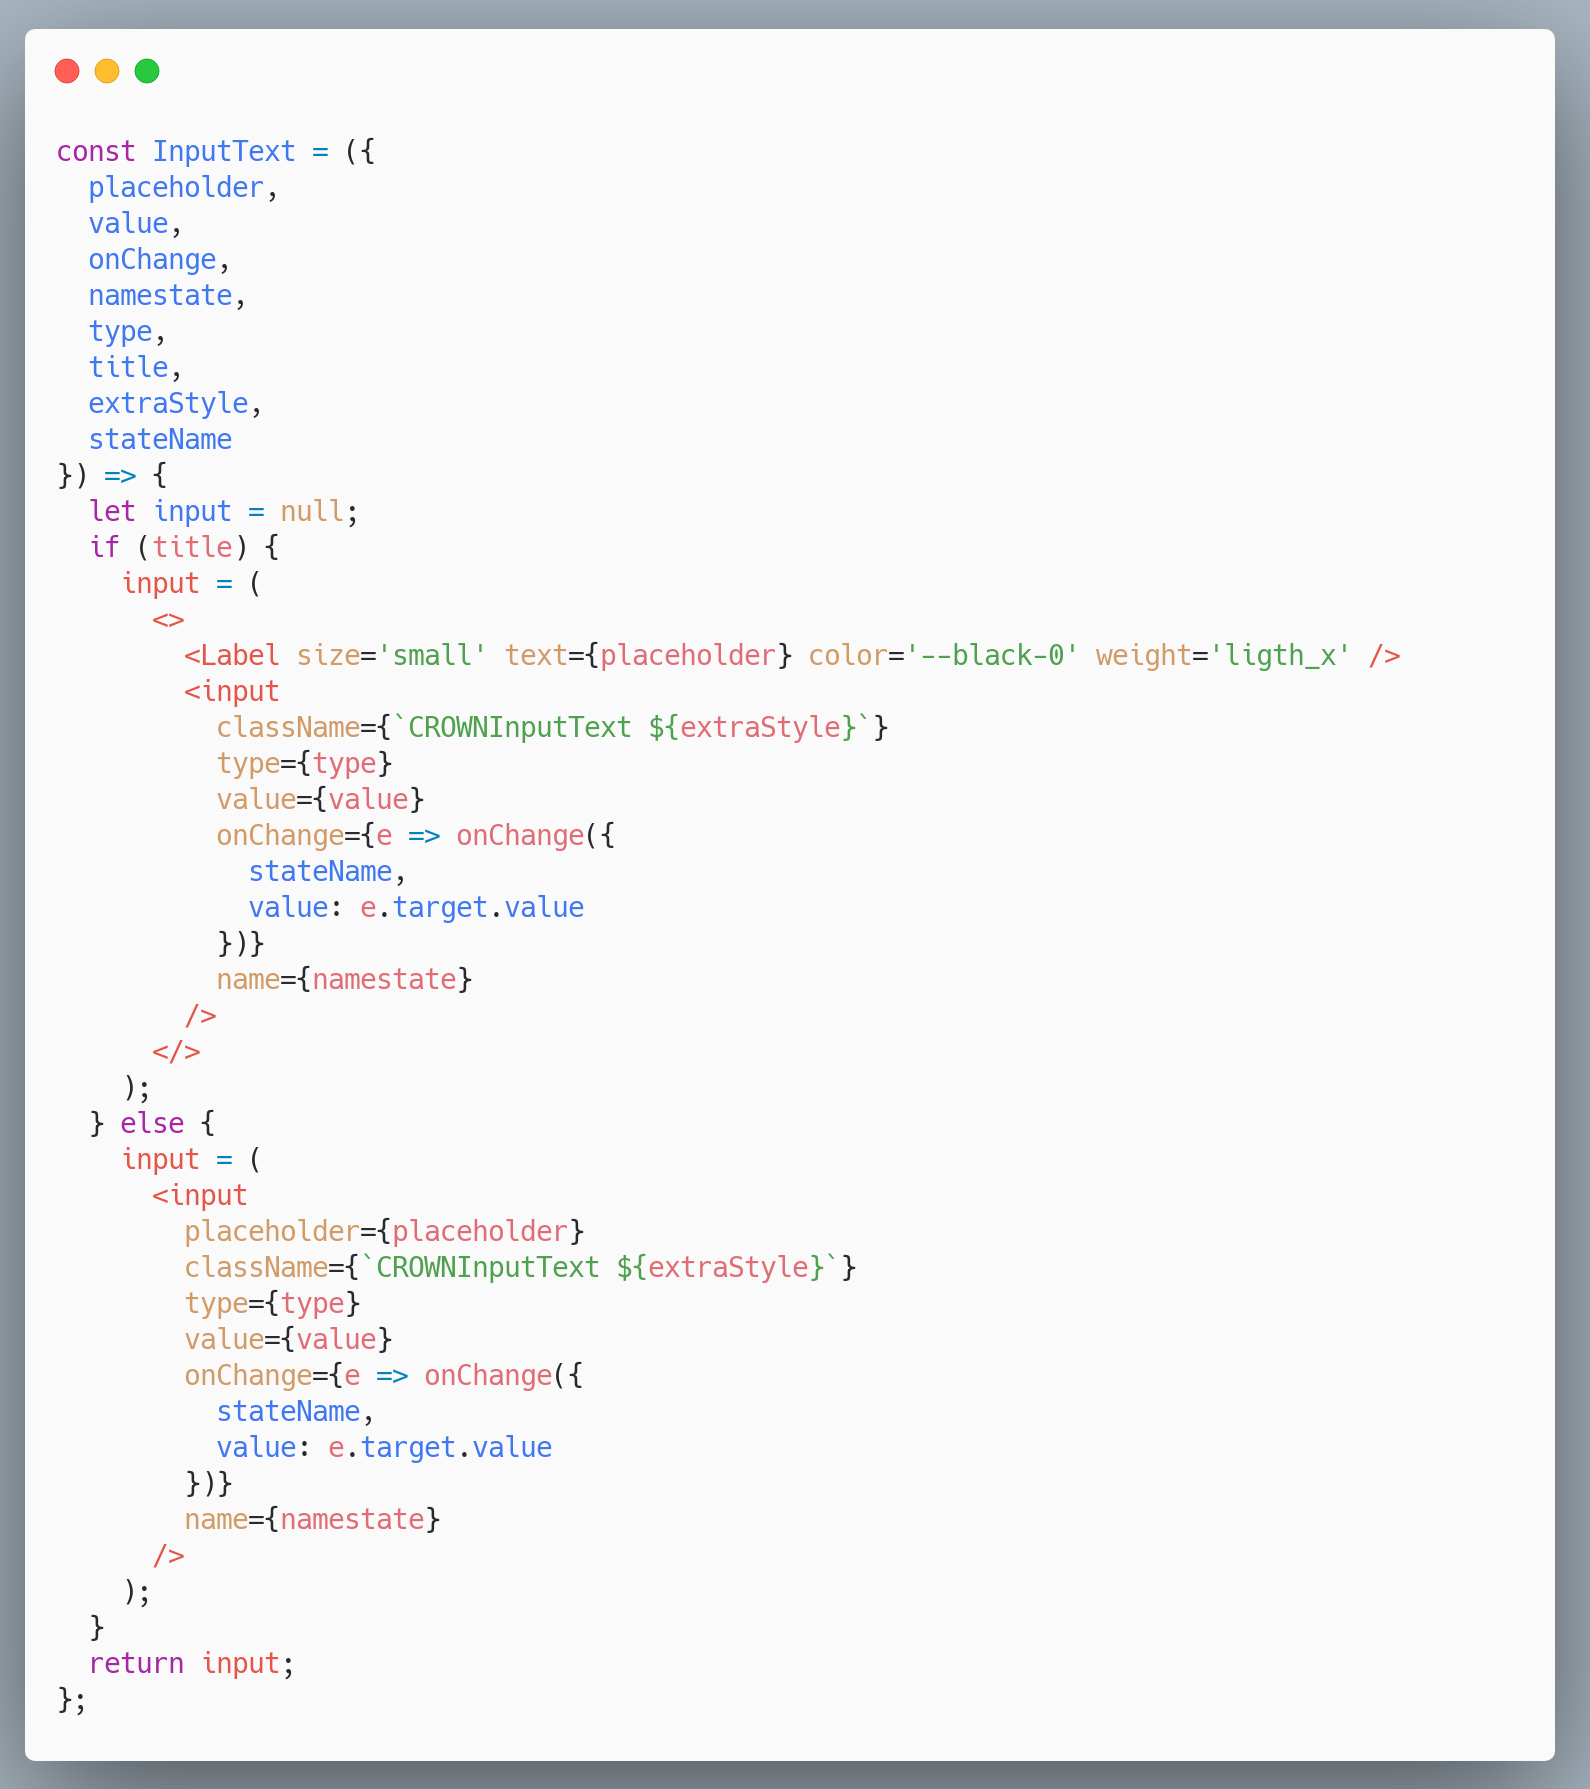
\includegraphics[width=1\textwidth]{./Imagenes/carbon-12.png}
    \caption[Código fuente del elemento InputText]{Código fuente del elemento InputText}
    \end{figure}
\newline
\newline



\subsection{Elemento Drop Down}
\subsection{Elemento Radio Button}
\subsection{Elemento Switch}
\subsection{Elemento Table}
\subsection{Elemento Check Box}
\subsection{Elemento Image}


				
			\section {Test }
				Para garantizar el correcto funcionamiento de cada uno de los componentes se diseñan una serie de test para comprobar el comportamiento. Para esto se usará una librería llamada Jest \cite{jest} (Getting Started · Jest), para instalarla se debe ejecutar el siguiente comando.
\newline
\begin{figure}[H]
    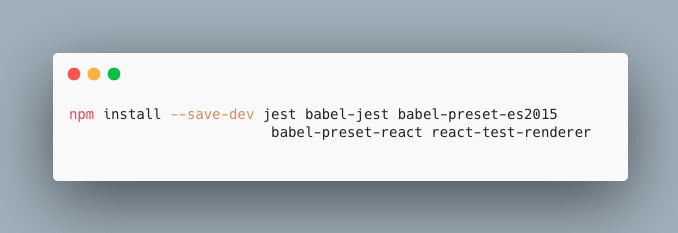
\includegraphics[width=1\textwidth]{./Imagenes/8.39t.png}
    \caption[Instalar dependencias]{Instalar dependencias}
    \end{figure}
\newline
Las dependencias instaladas con el comando anterior solo son usadas durante el desarrollo.

Dentro del directorio src debemos crear un subdirectorio llamado Test.
\newline
\begin{figure}[H]
    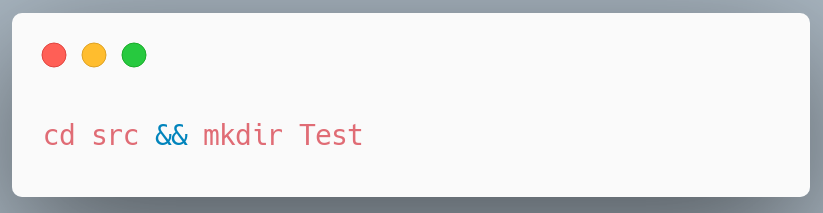
\includegraphics[width=1\textwidth]{./Imagenes/8.40t.png}
    \caption[Crear directorio]{Crear directorio}
    \end{figure}
\newline
Y dentro de este directorio crearemos un archivo por cada uno de los componentes llamado de la siguiente manera.
\begin{figure}[H]
   Nombre del Componente + . + test + . + js
    \centering
    \end{figure}
    
 Dentro de este se tendrán un código para asegurar el funcionamiento, por ejemplo para el componente Button se diseñó el siguiente test.
 \newline
\begin{figure}[H]biblioteca
    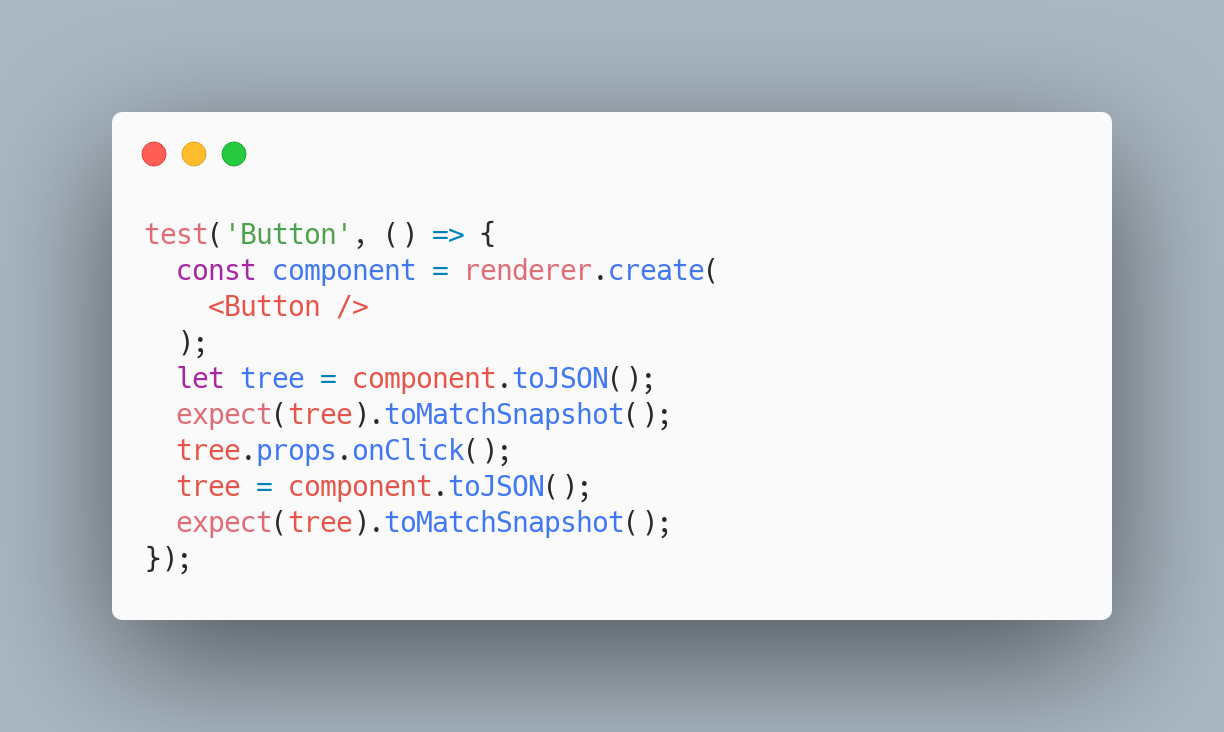
\includegraphics[width=1\textwidth]{./Imagenes/8.41t.png}
    \caption[Test del componente Button]{Test del componente Button}
    \end{figure}
\newline

El cual crea un componente, después crea una copia del resultado, y cada que se ejecute el test se debe comparar con la copia creada.
La segunda parte del test hacé click en el botón y verifica el funcionamiento.

Para poder ejecutar el todos los test, se debe agregar el siguiente comando en el archivo packeage.json.
 \newline
\begin{figure}[H]
    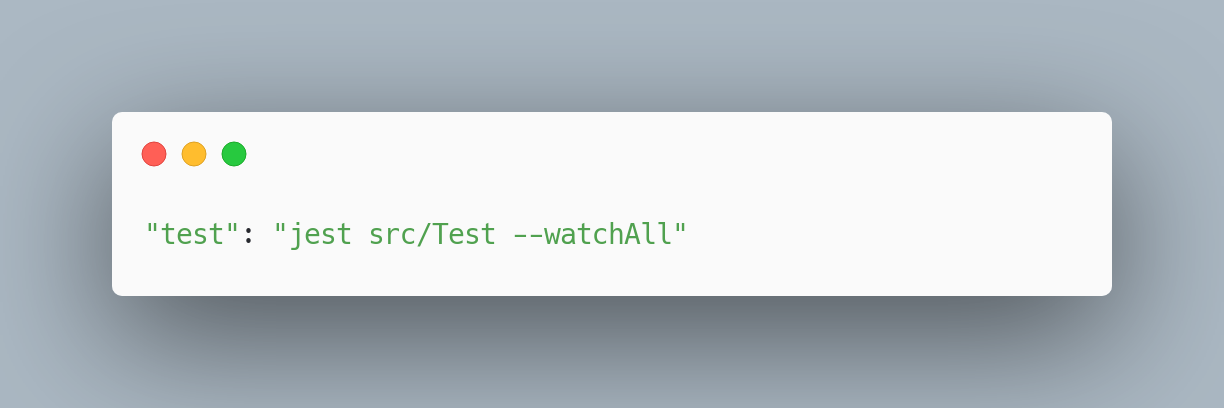
\includegraphics[width=1\textwidth]{./Imagenes/8.42t.png}
    \caption[Agregar comando]{Agregar comando}
    \end{figure}
\newline
\clearpage
				
			\section {Publicación de la biblioteca en NPM }
				Finalmente una vez tenemos todos los elementos completamente desarrollados y terminados debemos proceder a publicar nuestra librería para que esta sea de uso libre para toda la comunidad de desarrolladores de software Web que implementan Node.

Debemos configurar el nombre de nuestro paquete que será con el que las personas pueden encontrarlo, esta librería se llama "crown components", este nombre se especifica en el archivo package.json en el directorio raíz de nuestro proyecto en la llave “name”.

Tenemos que ingresar con nuestra cuenta desde la terminal con el siguiente comando.
  \newline
    \begin{figure}[H]
    \centering
    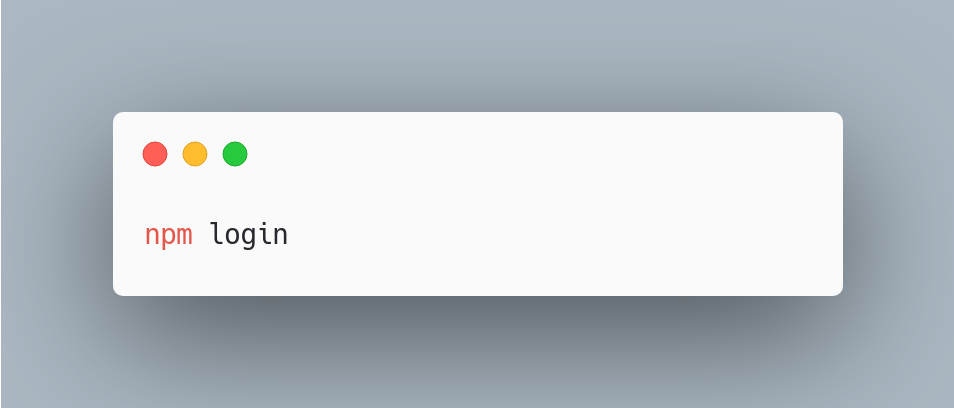
\includegraphics[width=0.7\textwidth]{./Imagenes/8.39.png}
    \caption[ingresar a nuestra cuenta]{Ingresar a nuestra cuenta}
    \end{figure}
    
    Este comando solicitará el nombre de usuario, contraseña y correo electrónico de nuestra cuenta de NPM, es necesario tener una cuenta previamente creada.

Una vez con la sesión iniciada en la terminal es posible publicar nuestro paquete con el siguiente comando.
  \newline
    \begin{figure}[H]
    \centering
    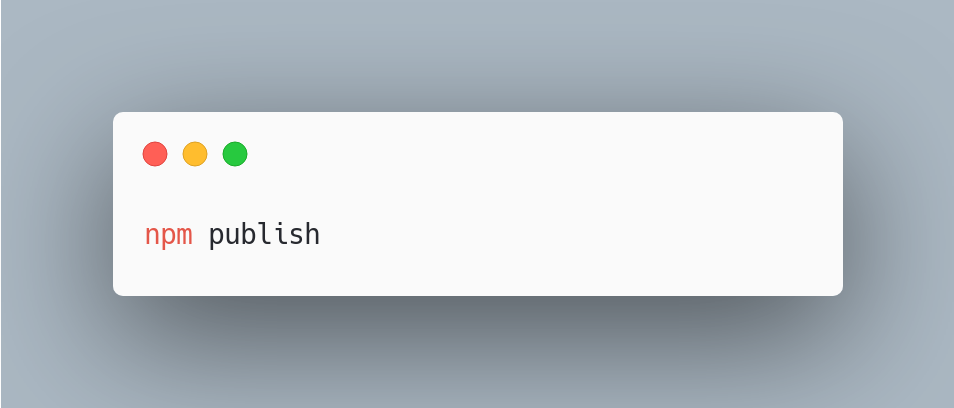
\includegraphics[width=0.7\textwidth]{./Imagenes/8.40.png}
    \caption[Publicar paquete]{Publicar paquete}
    \end{figure}
        Y con esto tenemos nuestra librería publicada.
    \clearpage
    

			
			\section {Diferencia entre el uso nativo de React y esta biblioteca}
				
Hasta este punto se tiene la librería publicada en el gestor de paquetes NPM, pero aún no se tiene conciencia sobre la diferencia que existe entre usar esta librería o implementar React de manera normal.
A continuación se tiene un ejemplo de cómo se implementaría el Front-End para mostrar la lista de calificaciones de un grupo de estudiantes con React.

Queremos tener una vista que tenga el título “Lista de calificaciones” con una tabla que tenga el nombre, el semestre y tres calificaciones parciales. 

Supongamos que al hacer una petición al servidor Back-end ( Esta librería no cubre la manera directa de interactuar con el Back-end ), y nos regresa como respuesta un array con los datos y calificaciones de los alumnos como se muestra en la siguiente imagen,el array llamado ALUMNOS. También tenemos un array llamado HEADER el cual tiene la cabecera de la tabla.

 \newline
     \begin{figure}[H]
    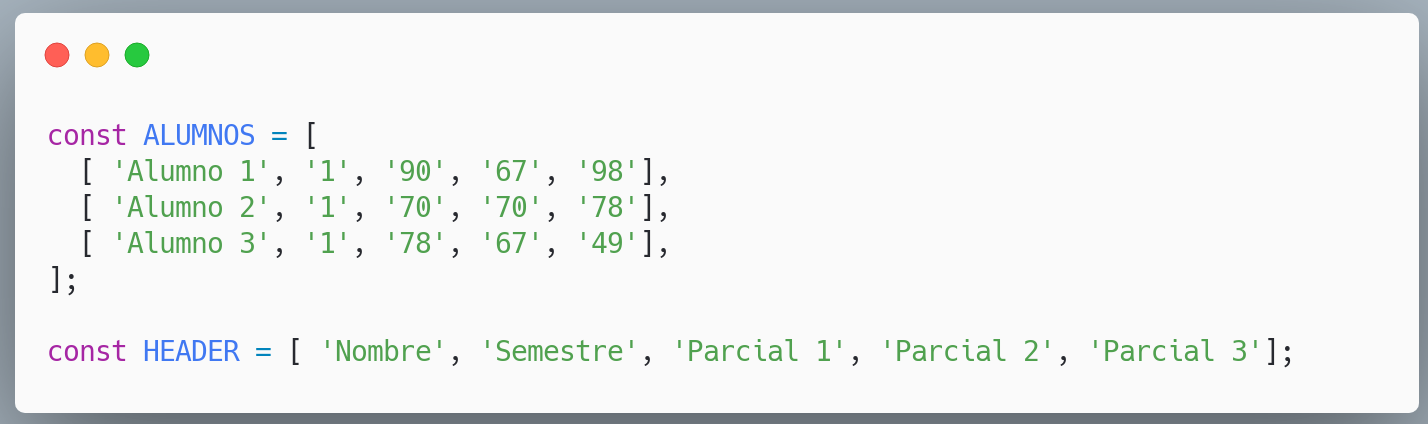
\includegraphics[width=1\textwidth]{./Imagenes/array.png}
     \caption[Crear nuevos directorios]{Array de datos}
         \end{figure}
    \newline

En React tendríamos el siguiente código para poder mostrar en pantalla una tabla.

 \newline
     \begin{figure}[H]
    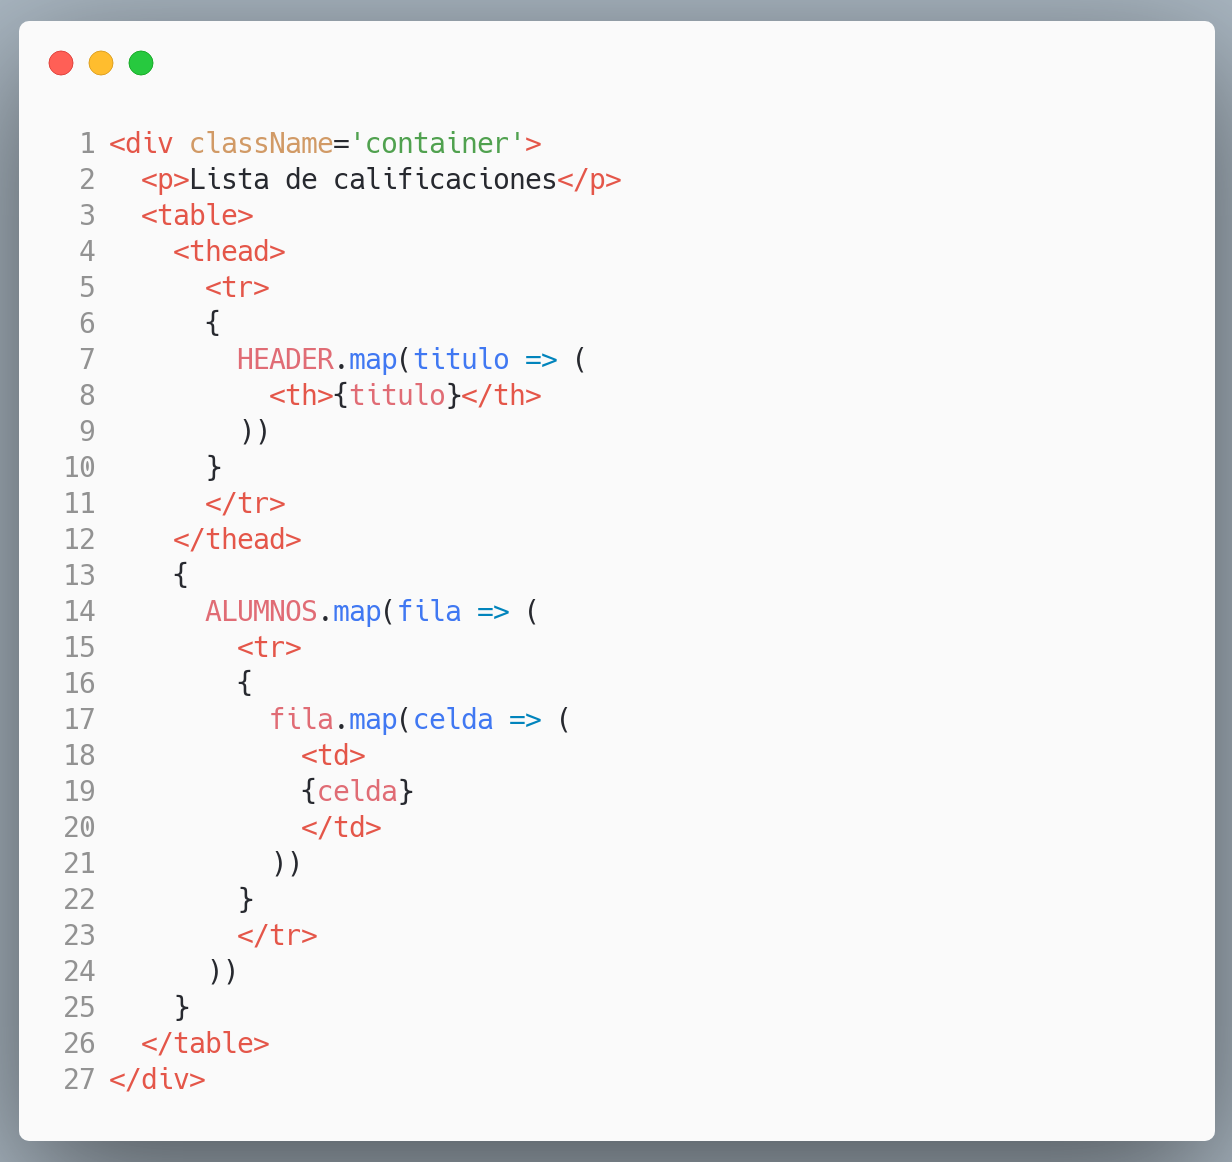
\includegraphics[width=1\textwidth]{./Imagenes/table-react.png}
     \caption[Crear nuevos directorios]{Array de datos}
         \end{figure}
    \newline
    
    En la línea dos, tenemos el título de la vista, a partir de la línea tres tenemos la tabla, la primera parte ( línea cuatro) hacemos la cabecera de la tabla, para esto tenemos que recorrer el array llamado HEADER con ayuda de la función de JavaScript llamada map.

Después en la línea trece, formamos el contenido de la tabla, tenemos que recorrer el array ALUMNOS, primero se recorre fila por fila, y en la línea diecisiete dada una fila, se recorre celda por celda.

Para que esto luzca de manera deseada se tiene el siguiente CSS.

 \newline
     \begin{figure}[H]
    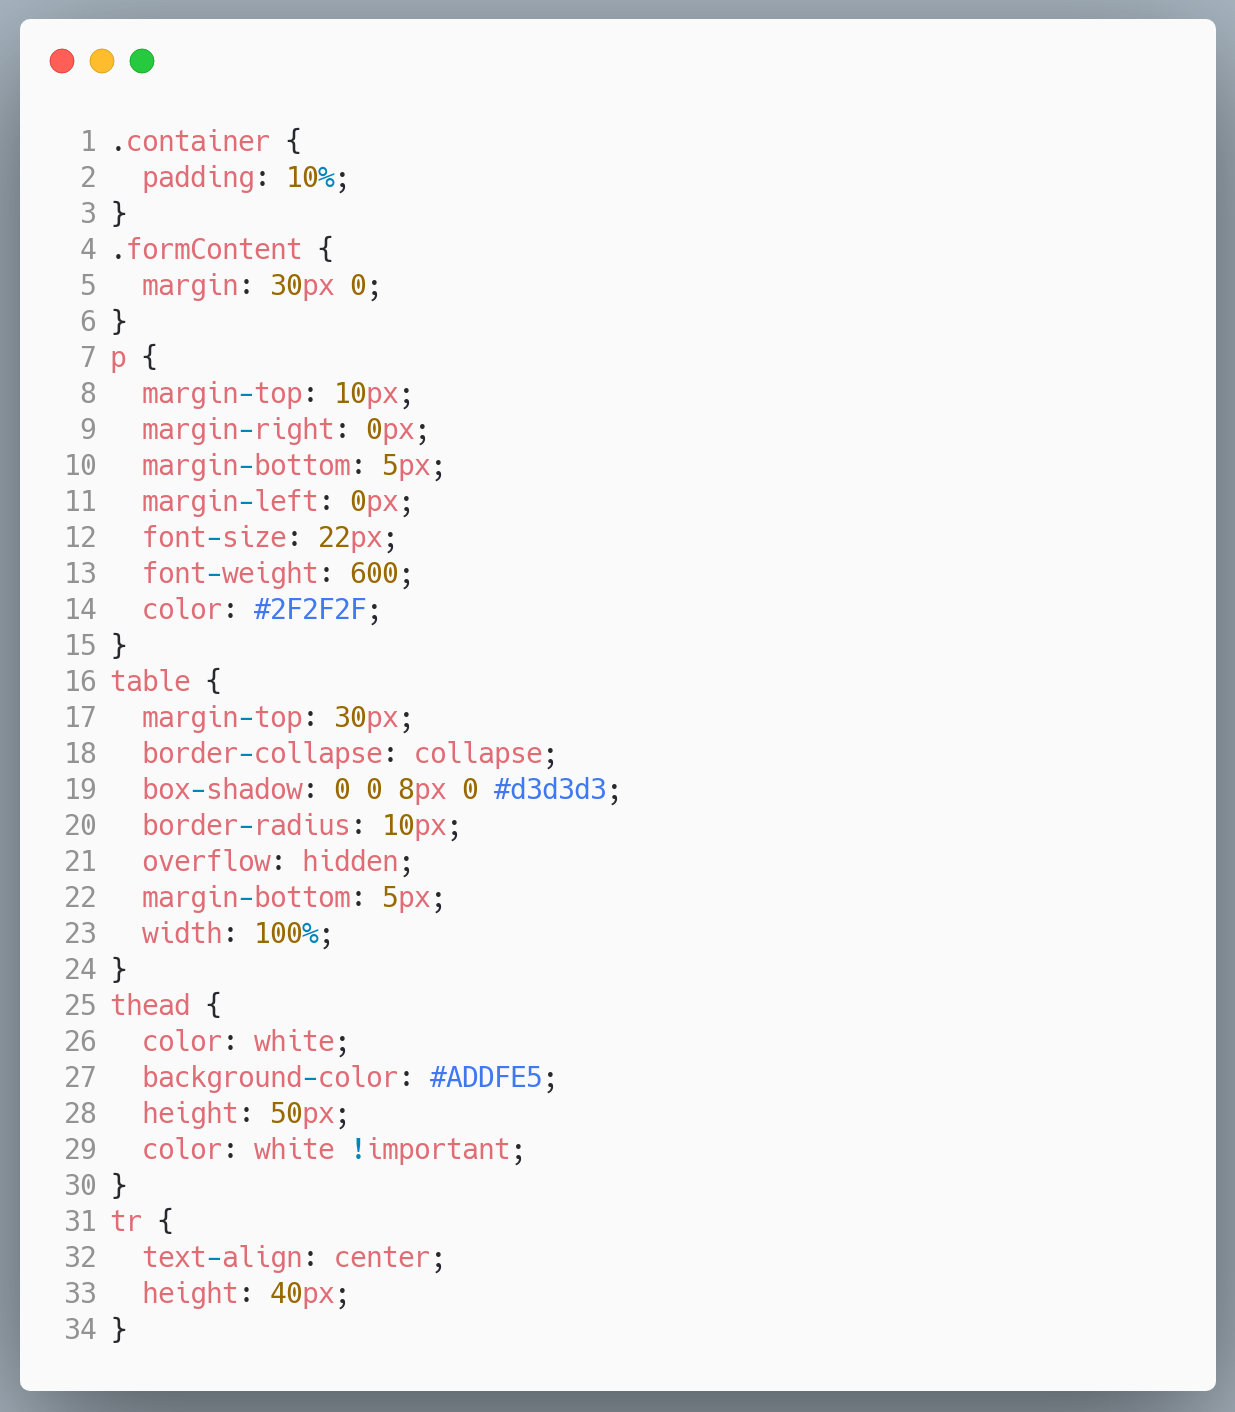
\includegraphics[width=1\textwidth]{./Imagenes/table-css.png}
     \caption[Crear nuevos directorios]{Array de datos}
         \end{figure}
    \newline
    
    Y así tenemos el siguiente resultado.
    
     \newline
     \begin{figure}[H]
    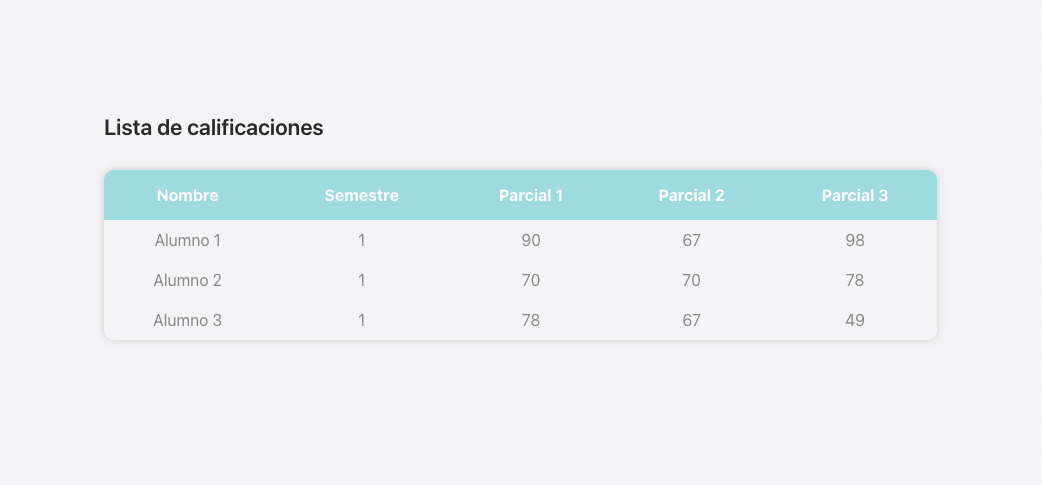
\includegraphics[width=1\textwidth]{./Imagenes/table-res.png}
     \caption[Crear nuevos directorios]{Array de datos}
         \end{figure}
    \newline
    
    Con nuestra librería evitamos el trabajo de formar desde cero la tabla, y no se tiene que dar estilos  CSS, Para tener el resultado anterior no tenemos que hacer nada, más que pasarle los datos de la cabecera y el cuerpo de la tabla de la siguiente manera.
         \newline
     \begin{figure}[H]
    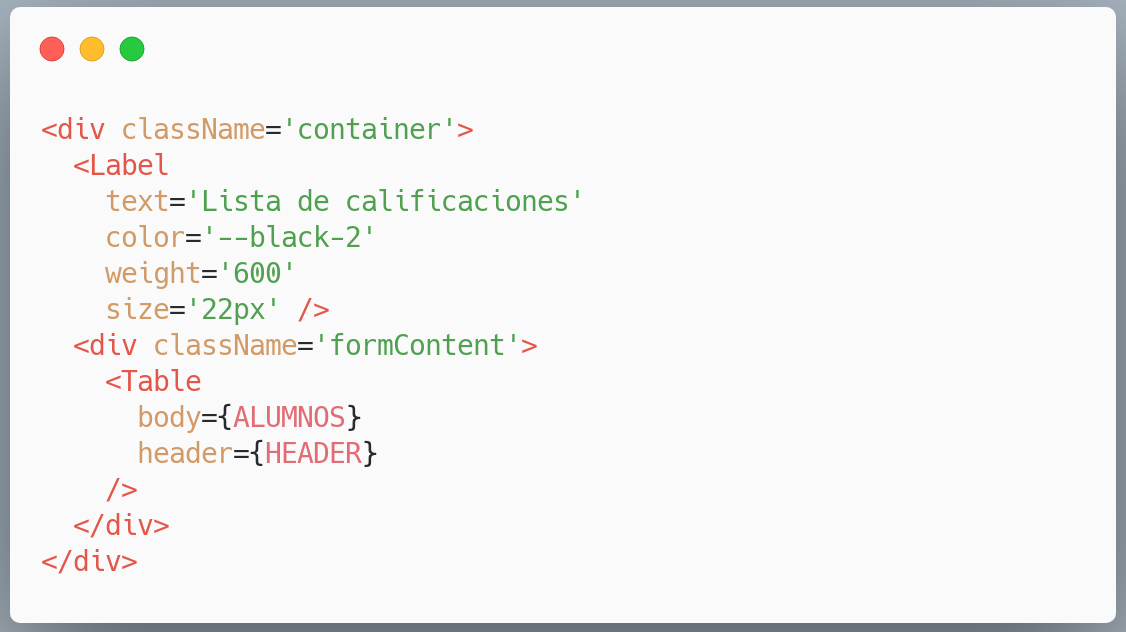
\includegraphics[width=1\textwidth]{./Imagenes/table-crown.png}
     \caption[Crear nuevos directorios]{Array de datos}
         \end{figure}
    \newline
    
    Con el código anterior, estamos usando la librería aquí desarrollada, al inicio tenemos el componente Label al cual le damos parámetros como el tamaño de la letra, su peso y el texto a mostrar que en este caso es “Lista de calificaciones”. Y después tenemos el componente Table, al cual solo le pasamos los arrays ALUMNOS para el cuerpo de la tabla y HEADER para la cabecera de la tabla.
    
    
			
		
		\chapter {Pruebas y Resultados}
			Con el desarrollo de la librería ya es posible hacer la implementación de un proyecto el cual ya usa React.
A continuación se ejemplifica el uso de la librería paso a paso.

Existe una herramienta que nos permite crear el esqueleto de una web basada en React. \cite{CRA} esta es desarrollada y mantenida por Facebook, de la cual partiremos para crear una web en la que probaremos la librería.

Instalaremos la herramienta llamada Create React App con el siguiente comando.
\newline
\begin{figure}[H]
    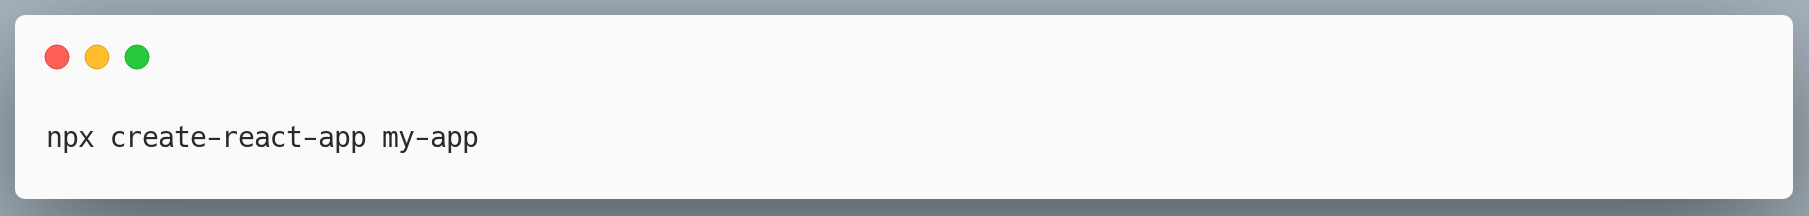
\includegraphics[width=1\textwidth]{./Imagenes/9.1.png}
    \caption[Instalar Create React App]{Instalar Create React App}
    \end{figure}
\newline

Crearemos la web llamada ejemplo-1 con el siguiente comando.
\newline
\begin{figure}[H]
    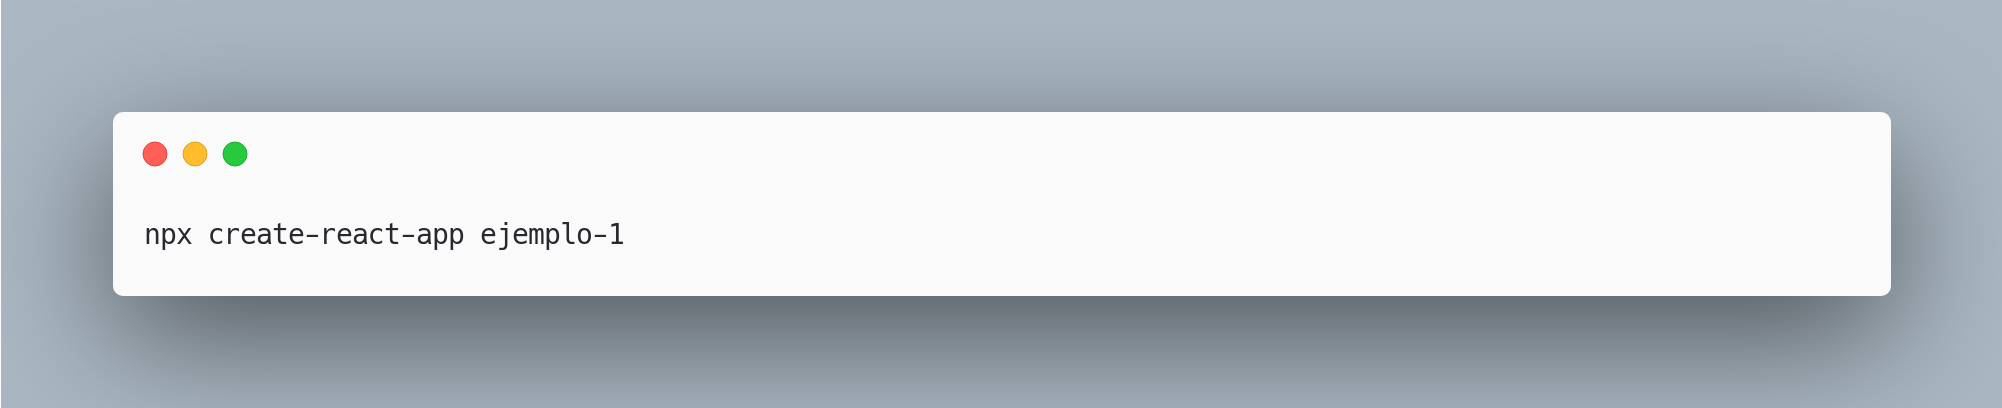
\includegraphics[width=1\textwidth]{./Imagenes/9.2.png}
    \caption[Crear una nueva app]{Crear una nueva app}
    \end{figure}
\newline

El comando nos generará los siguientes directorios.
\newline
\begin{figure}[H]
    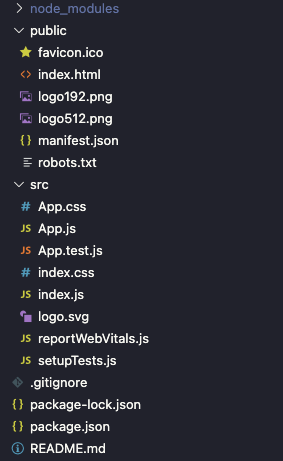
\includegraphics[width=0.5\textwidth]{./Imagenes/9.3.png}
   \centering 
    \caption[Directorios al crear una nueva app]{Directorios al crear una nueva app}
    \end{figure}
\newline

Para poder probar nuestra librería debemos a indicar a la app ejemplo-1 que use la dependencia instalándola con el siguiente comando.\newline
\newline
\begin{figure}[H]
    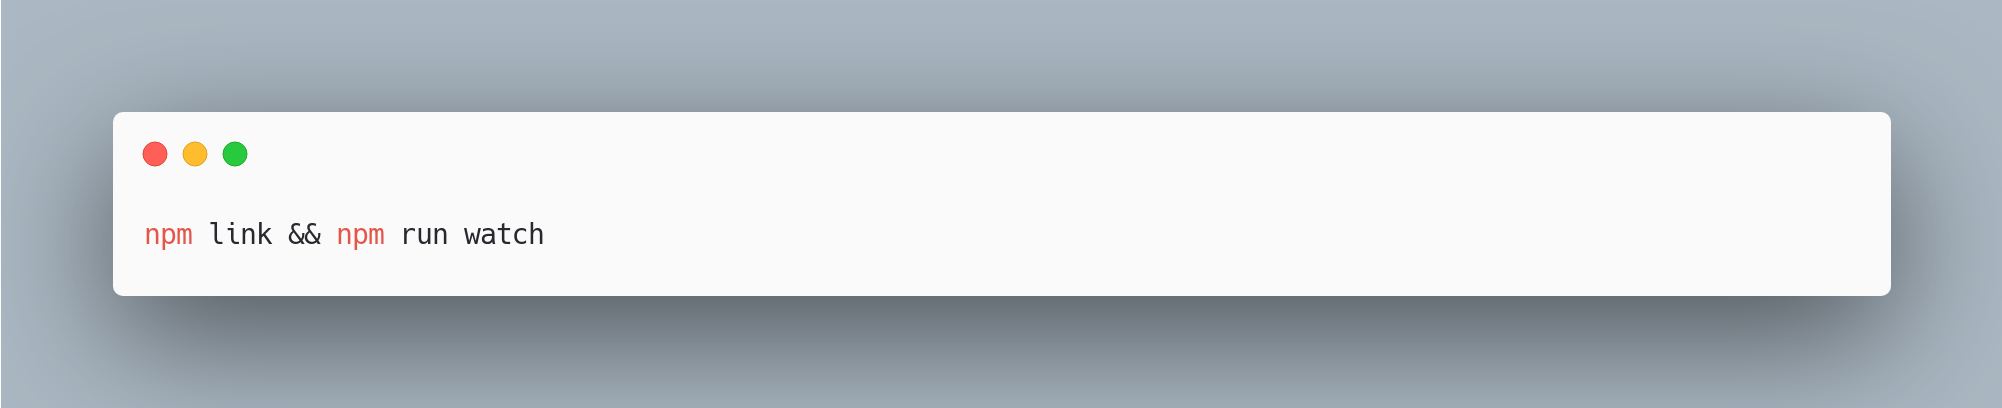
\includegraphics[width=1\textwidth]{./Imagenes/9.4}
   \centering 
    \caption[Instalando nuestra librería]{Instalando nuestra librería}
    \end{figure}
\newline

Ahora basta incluirlo como se agrega cualquier dependencia de node, basta con agregar cualquiera de los elementos aquí desarrollados. 

Crearemos dos ejemplos simples para mostrar el funcionamiento de la librería.
El primero consta de un formulario el cual solicita nombre, correo electronico y contraseña, esto con el objetivo de registrar un usuario para que tenga un correo institucional, también se le solicitará si la cuenta estará activa al momento de crearla.

Para esto debemos importar nuestros componentes de la siguiente manera.
\newline
\begin{figure}[H]
    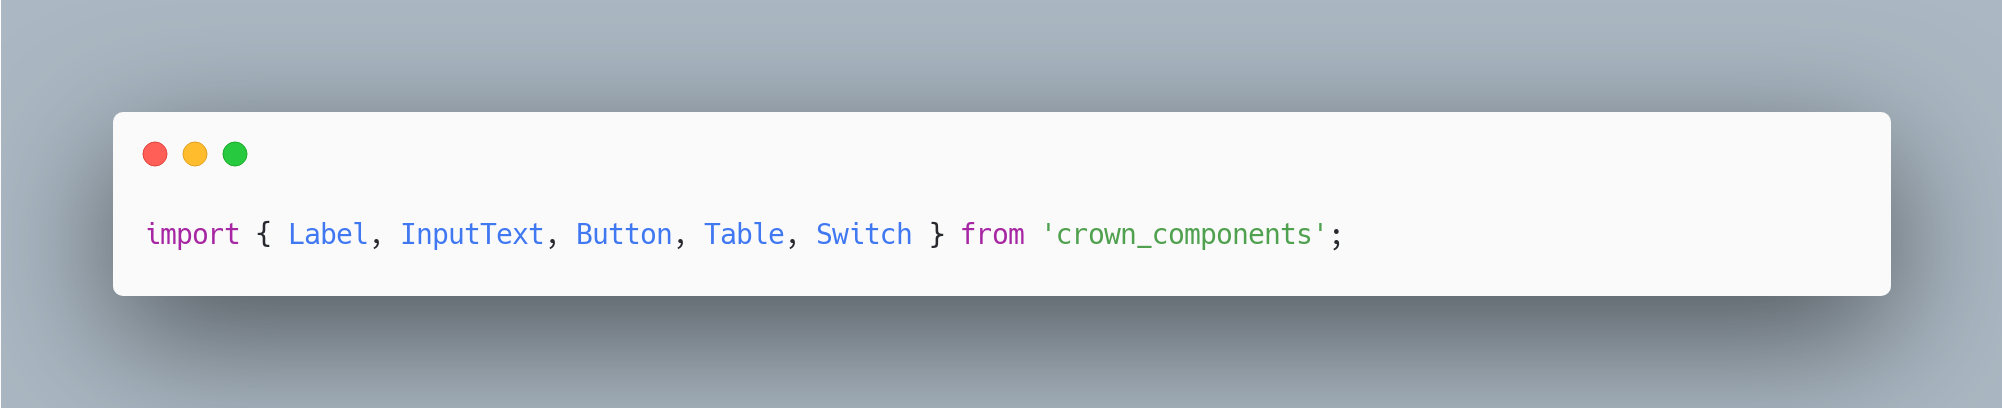
\includegraphics[width=1\textwidth]{./Imagenes/9.6}
   \centering 
    \caption[Implementación la librería]{Implementación la librería}
    \end{figure}
\newline

Después en el estado de React debemos agregar algunos campos para almacenar la información del formulario como se muestra en la siguiente figura.
\newline
\begin{figure}[H]
    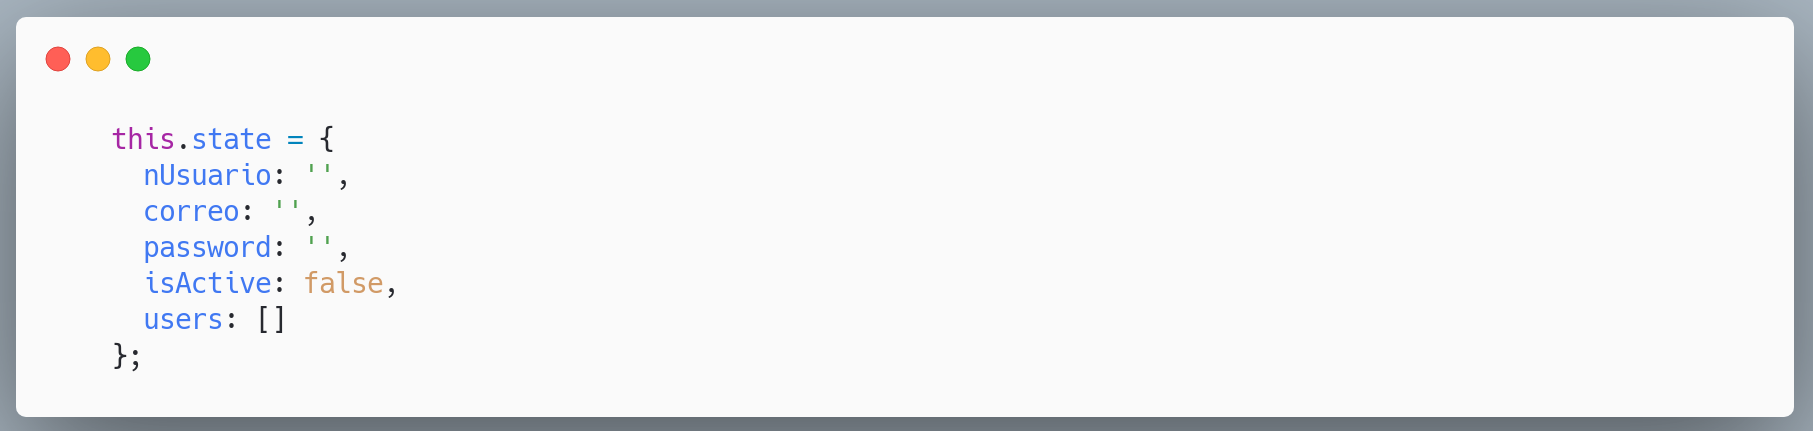
\includegraphics[width=1\textwidth]{./Imagenes/9.7}
   \centering 
    \caption[Agregar campos al estado de React]{Agregar campos al estado de React}
    \end{figure}
\newline
Los datos se usarán para:

  \begin{itemize}
   \item \textbf{ nUsuario:} Nombre de usuario del nuevo registro.
   \item \textbf{ correo:} Correo del usuario.
   \item \textbf{ password:} Contraseña del usuario.
   \item \textbf{ isActive:} Activar la cuenta al crearla.
   \item \textbf{ users:} Usuarios registrados, esto simulando nuestra base de datos.
  \end{itemize}

En la siguiente imagen se muestra el código necesario para desplegar en pantalla el formulario requerido así como una tabla para mostrar los usuarios registrados.

\newline
\begin{figure}[H]
    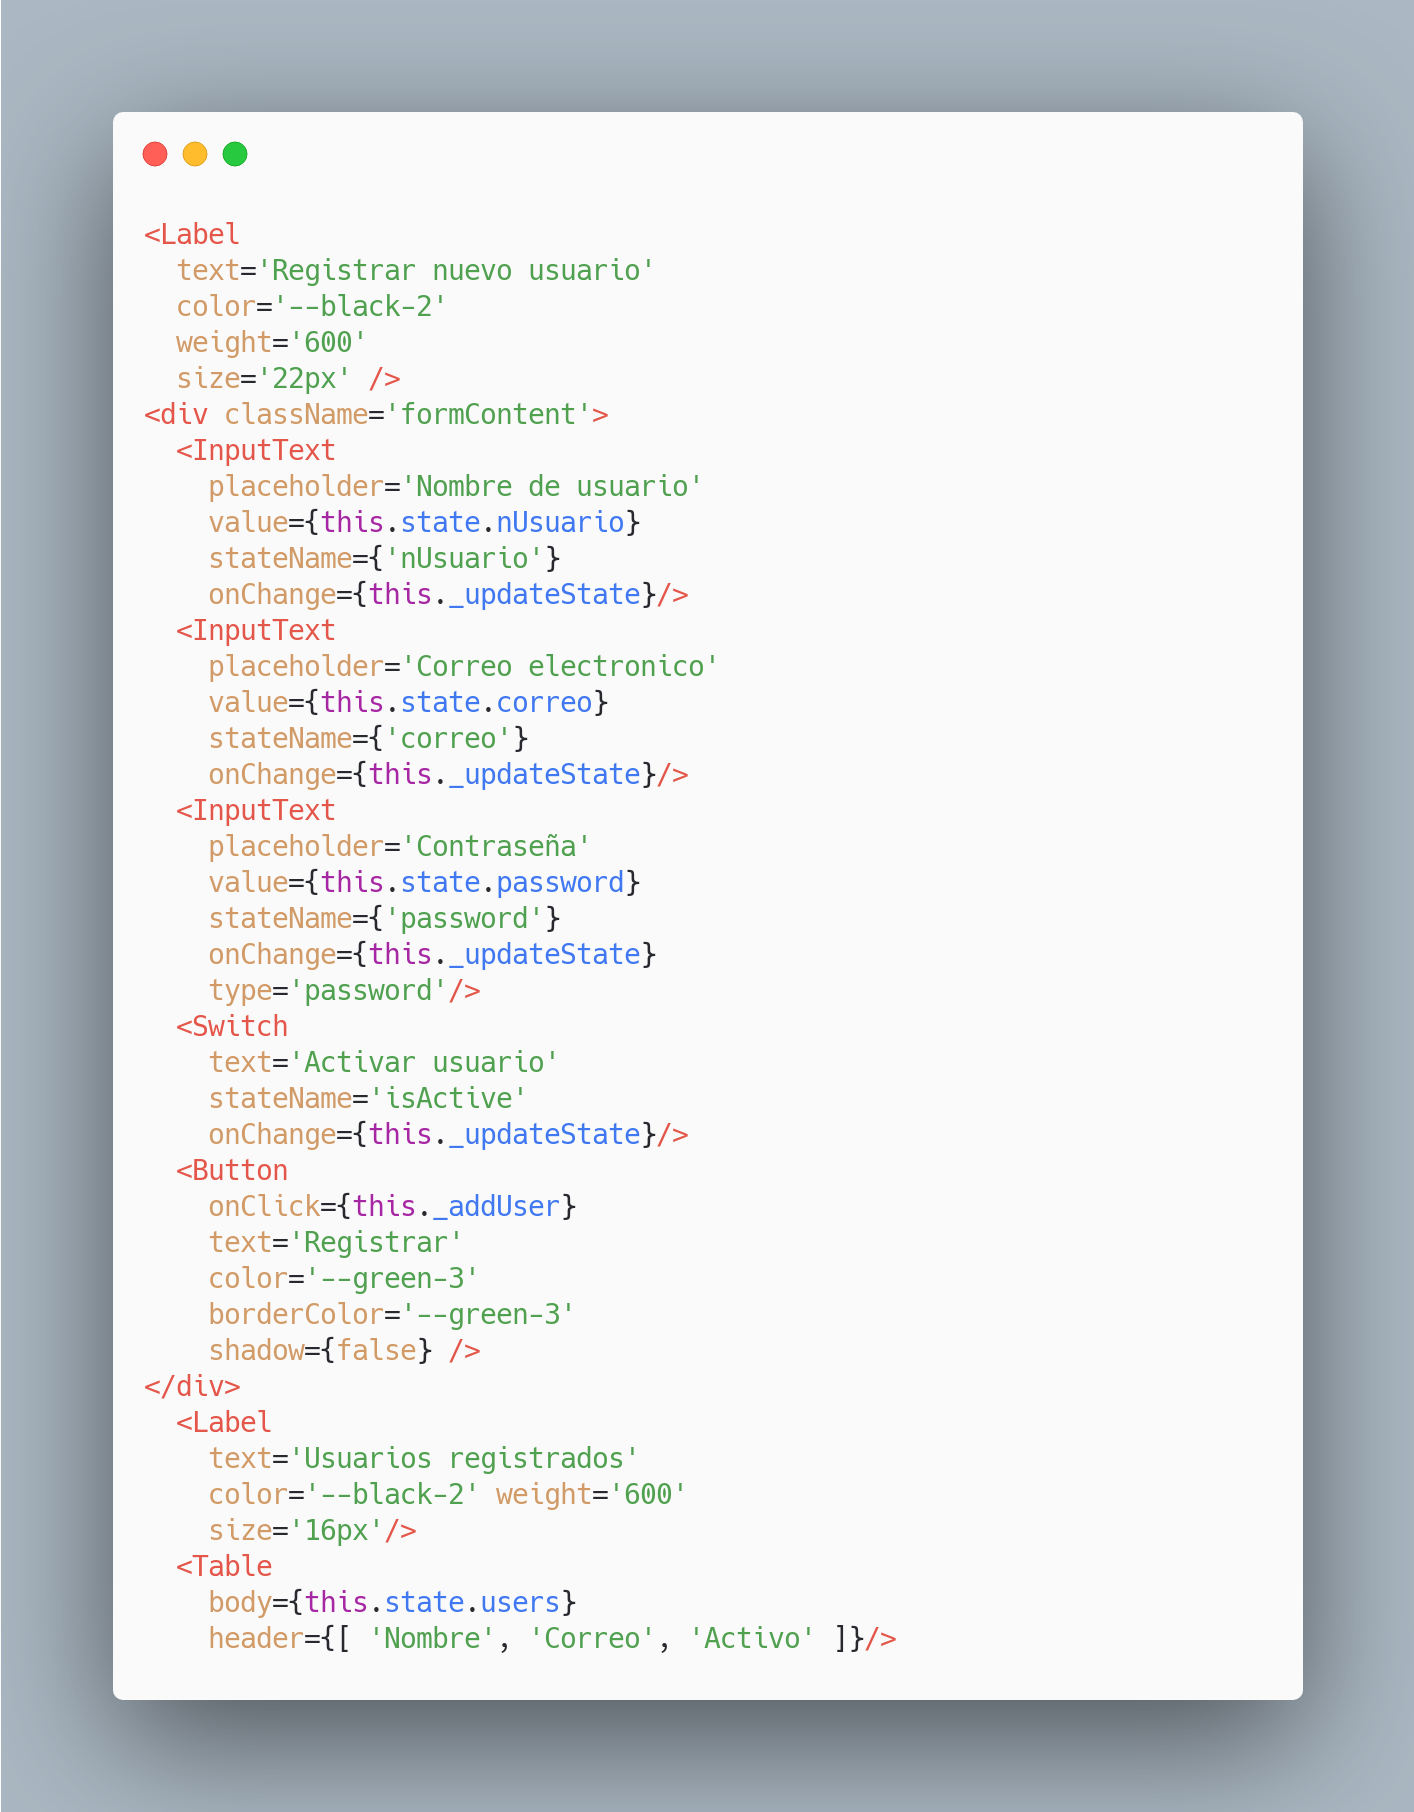
\includegraphics[width=1\textwidth]{./Imagenes/9.8}
   \centering 
    \caption[Código para maquetar]{Código para maquetar}
    \end{figure}
\newline

El código contiene al inicio un componente Label el cual muestra en pantalla un texto dado con las especificaciones de preferencia, se le da un tamaño de letra y color del texto. Después siguen una serie de InputText los cuales son la entrada de datos para el nombre de usuario, correo electronico  y contraseña, Estos tienen parámetros que son importantes de mencionar ya se son indispensables para el correcto funcionamiento como son:
placeholder: Es el texto que se mostrará en el campo de texto antes de que se introduzca un dato, para dar una pista del dato solicitado.
value: Es el estado de React en el que se almacenará cuando ocurra un cambio.
stateName: Es la forma en como es llamado en el estado de react ( Ejemplo. en este caso sería alguna de las llaves que se muestran en la Figura 9.6 ).
onChange: Es la función que se activará cuando algún dato se actualice.

El último parámetro onChange es una función simple como la que se muestra a continuación. 

\newline
\begin{figure}[H]
    \includegraphics[width=1\textwidth]{./Imagenes/9.9}
   \centering 
    \caption[Función para actualizar el estado de React]{Función para actualizar el estado de React}
    \end{figure}
\newline

Esta función es única para cualquiera de los componentes de la librería, ya que están diseñados para que cuando se actualicen, regresen el nombre por el cual están identificados en el estado de React para saber que dato actualizar  y el nuevo valor.
Finalmente se tiene el componente Button y Table. El componente Button tiene un parámetro, onClick el cual envía una función que se ejecutará cuando se haga click. Esta función actualiza el parámetro del estado llamado users que almacena de manera no persistente los usuarios que se vayan agregando.
El componente Tabla recibe un arreglo para la cabecera y un arreglo de arreglos para el cuerpo de la tabla.


A continuación se muestra el resultado que se tendría con unas escasas líneas de código usando la librería.
\newline
\begin{figure}[H]
    \includegraphics[width=1\textwidth]{./Imagenes/9.10}
   \centering 
    \caption[Resultado final]{Resultado final}
    \end{figure}
\newline
También se tiene el resultado después de agregar algunos usuarios.
\newline
\begin{figure}[H]
    \includegraphics[width=1\textwidth]{./Imagenes/9.11}
   \centering 
    \caption[Resultado final al agregar usuarios]{Resultado final al agregar usuarios}
    \end{figure}
\newline

En seguida se muestra otro ejemplo que figura un restaurante en el cual se muestran los platillos que se venden, con la posibilidad de filtrarlos si son bebidas o tragos.

En el estado de React se tiene solamente un dato, este es el modo por el cual se están filtrando los datos.
\newline
\begin{figure}[H]
    \includegraphics[width=0.7\textwidth]{./Imagenes/9.11-2}
   \centering 
    \caption[Filtro en el estado de React]{Filtro en el estado de React}
    \end{figure}
\newline

El código para maquetar los platillos es el siguiente el cual puede ser usado por ejemplo para la web de un restaurante la cual recibe los datos de algún otro servicio web.
El código de la siguiente web cuenta con elemento DropDown que permite filtrar para mostrar comida o tragos las opciones posibles para mostrar son enviadas por el parámetro options, stateName es el nombre de llave que almacena la opción por la que se filtra, y también se tiene optionSelected que es en si el filtro.

Después se tiene un ciclo en el que se agrega cada uno de los platillos, el componente Card recibe el título de la tarjeta, la imagen y el contenido.
\newline
\begin{figure}[H]
    \includegraphics[width=1\textwidth]{./Imagenes/9.12.png}
   \centering 
    \caption[Código para mostrar los platillos]{Código para mostrar los platillos}
    \end{figure}
\newline

En las siguientes imágenes se muestra el resultado del código.
\newline
\begin{figure}[H]
    \includegraphics[width=1\textwidth]{./Imagenes/9.13.png}
   \centering 
    \caption[Filtrar por comida]{Filtrar por comida}
    \end{figure}
\newline

\newline
\begin{figure}[H]
    \includegraphics[width=1\textwidth]{./Imagenes/9.14.png}
   \centering 
    \caption[Filtrar por bebida]{Filtrar por bebida}
    \end{figure}
\newline

También se cuenta con el elemento Modal que puede ser usado como confirmación cuando el comprador presiona el botón para comprar un platillo.
\newline
\begin{figure}[H]
    \includegraphics[width=1\textwidth]{./Imagenes/9.15.png}
   \centering 
    \caption[Confirmación de pedido]{Confirmación de pedido}
    \end{figure}
\newline


		
		\chapter {Conclusiones Y Recomendaciones}
			Una vez el desarrollo de la biblioteca finalizado, y la herramienta publicada, se recomienda usar como documentación las tablas de propiedades que se encuentran dentro del capítulo 8.2, tablas las cuales muestran las propiedades que pueden ser modificadas en cada uno de los componentes para su correcto funcionamiento.
También se recomienda mantener siempre la versión más reciente que se encuentre publicada.

Finalmente se concluye con el pensamiento de no reinventar la rueda ya que existen múltiples bibliotecas que nos agiliza nuestro trabajo, y es fácil encontrar bibliotecas que se adecuen a cualquier proyecto en el que estamos trabajando. Así hacemos que lo complejo sea decidir una biblioteca y no el desarrollo en sí mismo.

		
		\chapter {Fuentes de Información}
			\renewcommand{\bibname}{}
\patchcmd{\thebibliography}{\chapter*}{\section*}{}{}

\begin{thebibliography}{100} 

\bibitem{airbnb} Agrawal, K. (2019, May 4). Airbnb Javascript style guide — Key takeaways - Docon. Medium. https://medium.com/docon/airbnb-javascript-style-guide-key-takeaways-ffd0370c053

\bibitem{reactOreilly} Banks, A., & Porcello, E. (2017). Learning REACT Functional Web Development with REACT and Redux. O’Reilly.

\bibitem{scss} Coyier, C. (2013). SASS FOR WEB DESIGNERS. https://abookapart.com/products/sass-for-web-designers

\bibitem{axios}Cruz, R. (2019, November 1). Using Axios For HTTP Requests - Rafael Cruz. Medium. https://medium.com/@ralph1786/using-axios-for-http-requests-be9abb80795b

\bibitem{html} Danny Goodman. (1998). Dynamic HTML The Definitive Reference. 101 Morris Street, Sebastopol, CA 95472: O'REILLY.

\bibitem{frontEnd} Fu, C. (2016). Exploration of Web front-end development technology and optimization direction.

\bibitem{} Gaikovina Kula, R., Ouni, A., M. German, D., & Inoue, K. (2017, septiembre). On the Impact of Micro-Packages: An Empirical Study of the npm JAVASCRIPT Ecosystem. Osaka University, Japan. https://arxiv.org/abs/1709.04638

\bibitem{webPack} Gallegos, G. (2017, 20 octubre). Para que es Webpack? Medium. https://medium.com/tecninja/porque-usar-webpack-4a5004094455

\bibitem{CRA} Getting Started | Create React App. (s. f.). Create React App. https://create-react-app.dev/docs/getting-started/

\bibitem{jest} Getting Started · Jest. (s. f.). Jest. https://jest-bot.github.io/jest/docs/getting-started.html

\bibitem{} Hudson, P. (2016). Hacking with REACT [Libro electrónico]. http://www.hackingwithREACT.com/

\bibitem{javascript} JAVASCRIPT. (2020, 11 agosto). Documentación web de MDN. https://developer.mozilla.org/es/docs/Web/JAVASCRIPT

\bibitem{} K. White, S. (2020, 10 enero). The 10 most in-demand tech jobs for 2020 — and how to hire for them. CIO. https://www.cio.com/article/3235944/hiring-the-most-in-demand-tech-jobs-for-2018.html

\bibitem{mobileFirst} Mobile-first indexing best practices. (s. f.). Google Developers. https://developers.google.com/search/mobile-sites/mobile-first-indexing


\bibitem{} Open Source Initiative. (2006). The MIT license. 2015b.[Online]. Available: https://opensource. org/licenses/MIT.[Accessed 27 March 2017].


\bibitem{newTech} Popoter Pérez, G. J. (2016). Rediseño de aplicaciones utilizando las tecnologías modernas para el desarrollo web en su parte Front-end.


\bibitem{} Pozas, J. L. B. (2018, 11 enero). Las 10 profesiones de TI con mayor demanda en 2017. CIO MX. https://cio.com.mx/las-10-profesiones-ti-mayor-demanda-en-2017/

\bibitem{} ¿Qué es el open source? (2020). Red Hat. https://www.redhat.com/es/topics/open-source/what-is-open-source

\bibitem{react} REACT – A JAVASCRIPT library for building user interfaces. (s. f.). REACT. https://REACTjs.org

\bibitem{work} Riquelme, R. (2016, 17 octubre). Los 10 mejores trabajos en TI e Ingeniería. El Economista. https://www.eleconomista.com.mx/tecnologia/Los-10-mejores-trabajos-en-TI-e-Ingenieria-20161017-0053.html

\bibitem{publish} Rodriguez, M. A. (2019, 3 diciembre). Crear y publicar un paquete NPM en 4 sencillos pasos. Medium. https://medium.com/200-response/crear-y-publicar-un-paquete-npm-en-4-sencillos-pasos-8e7498b558a2

\bibitem{frontEnd2} Ruiz Inoue, K. (2020, 20 agosto). ¿Qué es el Desarrollo Front end, Back end y Fullstack? Medium. https://medium.com/deuk/qué-es-el-desarrollo-front-end-back-end-y-fullstack-2941b51afd1

\bibitem{stackOverflow} Stack Overflow Developer Survey 2020. (2020). Stack Overflow. https://insights.stackoverflow.com/survey/2020#overview

\bibitem{openSource} The Linux Foundation. (2018). Enterprise Open Source: A Practical Introduction [Libro electrónico].https://www.linuxfoundation.org/press-release/2018/08/free-ebook-enterprise-open-source-a-practical-introduction-teaches-enterprises-how-to-accelerate-open-source-efforts/

\bibitem{npm} What is npm. (2020). w3schools. https://www.w3schools.com/whatis/whatis_npm.asp

\bibitem{babel} What is Babel? · Babel. (2020). Babel. https://babeljs.io/docs/en/



\end{thebibliography}
			
		\chapter {Anexos}
		
\bibliography{library}

\end{document}